
\documentclass[11pt]{article}
\usepackage{jheppub}
\usepackage{epsfig}
\usepackage{amssymb}
\usepackage{amsmath}
\usepackage{tikz}
\usepackage{mathrsfs}
\usepackage{hyperref}
\usepackage{multirow}
\usepackage{scalerel}
\usepackage{mathtools}
\usepackage{textcomp}
\usepackage{color}
\usepackage[all]{xy}

\usetikzlibrary{calc}


\DeclareMathOperator{\B}{B}
\DeclareMathOperator{\Conf}{Conf}
\DeclareMathOperator{\Gr}{Gr}
\DeclareMathOperator{\Li}{Li}
\DeclareMathOperator{\sgn}{sgn}


\def\ket#1{\langle #1 \rangle}
\def\nl{\nonumber\\}
\def\nn{\nonumber}
\def\x{\mathcal{X}}
\def\xcoord{$\mathcal{X}$-coordinate }
\def\xcoords{$\mathcal{X}$-coordinates }
\def\a{\mathcal{A}}
\def\acoord{$\mathcal{A}$-coordinate }
\def\acoords{$\mathcal{A}$-coordinates }
\def\draftnote#1{{\bf [#1]}}
\def\flag{{\huge \color{red} \textinterrobang}}
\def\pdfeq#1{\texorpdfstring{$#1$}{a}}

\def\fd5{f_{D_5}}
\def\fa3{f_{A_3}}
\def\rn{R^{(2)}_n}
\def\rsev{R^{(2)}_7}

\def\bb2{B_2\wedge B_2}
\def\b3c{B_3 \otimes \mathbb{C}^*}


\def\drawPentagon{
\coordinate (P1) at (90:1);
\coordinate (P2) at (18:1);
\coordinate (P3) at (306:1);
\coordinate (P4) at (234:1);
\coordinate (P5) at (162:1);
\draw (P1) -- (P2) -- (P3) -- (P4) -- (P5) -- cycle;
}

\def\drawLabeledPentagon{
\coordinate (P1) at (90:1);
\coordinate (P2) at (18:1);
\coordinate (P3) at (306:1);
\coordinate (P4) at (234:1);
\coordinate (P5) at (162:1);
\draw (P1) -- (P2) -- (P3) -- (P4) -- (P5) -- cycle;
\draw (0,1.2) node {1};
\draw (1,.3) node[anchor=west] {2};
\draw (.5,-.9) node[anchor=west] {3};
\draw (-.5,-.9) node[anchor=east] {4};
\draw (-1,.3) node[anchor=east] {5};
}

\def\drawHexagon{
\coordinate (P1) at (90:1);
\coordinate (P2) at (30:1);
\coordinate (P3) at (330:1);
\coordinate (P4) at (270:1);
\coordinate (P5) at (210:1);
\coordinate (P6) at (150:1);
\draw (P1) -- (P2) -- (P3) -- (P4) -- (P5) -- (P6) -- cycle;
}


\def\drawLabeledHexagon{
\coordinate (P1) at (90:1);
\coordinate (P2) at (30:1);
\coordinate (P3) at (330:1);
\coordinate (P4) at (270:1);
\coordinate (P5) at (210:1);
\coordinate (P6) at (150:1);
\draw (P1) -- (P2) -- (P3) -- (P4) -- (P5) -- (P6) -- cycle;
\draw (0,1.2) node {1};
\draw (30:1.1) node[anchor=west] {2};
\draw (330:1.1) node[anchor=west] {3};
\draw (270:1.2) node {4};
\draw (210:1.1) node[anchor=east] {5};
\draw (150:1.1) node[anchor=east] {6};
}

\def\drawOctagon{
\coordinate (P1) at (45:1);
\coordinate (P2) at (90:1);
\coordinate (P3) at (135:1);
\coordinate (P4) at (180:1);
\coordinate (P5) at (225:1);
\coordinate (P6) at (270:1);
\coordinate (P7) at (315:1);
\coordinate (P8) at (359:1);
\draw (P1) -- (P2) -- (P3) -- (P4) -- (P5) -- (P6) -- (P7) -- (P8) -- cycle;
}


\def\mand#1{\scaleto{s}{4.6pt}_{\scaleto{#1}{5.2pt}}}
\def\EthreeJ{{}^{{\{a,b\}}_3} {\cal E}_8}
\def\EfourJ{{}^{{\{a,b\}}_4} {\cal E}_8}
\def\LiOneCalX#1#2{\text{Li}_1(-\mathfrak{X}_{#1,#2})}
\def\LiOneBarCalX#1#2{\text{Li}_1(-\overline{\mathfrak{X}}_{#1,#2})}

\newcommand{\cP}{{\cal P}}
\def\lr{\leftrightarrow}

\title{Cluster Subalgebra-Constructibility 
I: Novel Decompositions of the Seven-Particle Remainder Function} 

\author{John~Golden$^{1,2}$}
\author{and Andrew~J.~McLeod$^{2,3,4}$}


\affiliation{$^1$ Leinweber  Center for Theoretical Physics and
Randall Laboratory of Physics, Department of Physics,
University of Michigan
Ann Arbor, MI 48109, USA}

\affiliation{$^2$ Kavli Institute for Theoretical Physics, 
UC Santa Barbara, Santa Barbara, CA 93106, USA}

\affiliation{$^3$ SLAC National Accelerator Laboratory,
Stanford University, Stanford, CA 94309, USA}

\affiliation{$^4$ Niels Bohr International Academy, Blegdamsvej 17, 2100 Copenhagen, Denmark}

\abstract{The seven-particle remainder function in planar maximally supersymmetric Yang-Mills theory can be thought of as . We systematically investigate the ways in which the `nonclassical' part of  decomposed into the subalgebras of the Grassmannian Gr(4,7). We find it is possible to decompose }


\begin{document}
\maketitle

\section{Introduction}

A growing body of evidence suggests that cluster algebras (and their generalizations) have a central role to play in our understanding of multi-loop scattering amplitudes in the planar limit of ${\cal N} = 4$ supersymmetric Yang-Mills (SYM) theory. The most striking indication to this effect comes from the branch cut structure of its maximally-helicity-violating (MHV) amplitudes, which have now been computed to high loop orders in six- and seven-particle kinematics~\cite{Dixon:2013eka,Dixon:2014voa,Drummond:2014ffa,Caron-Huot:2016owq,Dixon:2016nkn}, and to two loops for any number of particles $n$~\cite{CaronHuot:2011ky}. Namely, all branch cuts in these amplitudes end at the vanishing loci of cluster coordinates on the Grassmannian Gr(4,$n$)~\cite{Golden:2013xva,Golden:2013lha,Golden:2014xqa,Golden:2014pua}, and---even more strikingly---their iterated discontinuities vanish unless sequentially taken across branch cuts associated with coordinates that appear together in at least one cluster in Gr(4,$n$)~\cite{Drummond:2017ssj,all_orders_adjacency}. All known next-to-MHV (NMHV) amplitudes in this theory share these remarkable properties~\cite{CaronHuot:2011kk,Dixon:2014iba,Drummond:2014ffa,Dixon:2015iva,Caron-Huot:2016owq,Dixon:2016nkn}, as do certain classes of Feynman integrals~\cite{Drummond:2010cz,Drummond:2017ssj,Bourjaily:2018aeq,Henn:2018cdp}, some of which have been computed to all loop orders~\cite{Caron-Huot:2018dsv}. While these amplitudes and integrals remain the simplest this theory has to offer, it remains suggestive that cluster algebras combinatorially realize so much of their analytic structure, thereby encoding their locality in a non-obvious way.

%In all its known loop-level amplitudes, the cluster coordinates on Gr(4,$n$) identify the location of branch cuts~\cite{Golden:2013xva,Golden:2013lha,Golden:2014xqa,Golden:2014pua,Dixon:2013eka,Dixon:2014voa,Dixon:2014iba,Drummond:2014ffa,Dixon:2015iva,Caron-Huot:2016owq,Dixon:2016nkn,Drummond:2017ssj}, as they do in Even more strikingly, the adjacent symbol entries of these (appropriately normalized) amplitudes and integrals are believed to involve only those cluster coordinates that appear together in clusters of Gr(4,$n$)~\cite{Drummond:2017ssj}.

The fact that cluster algebras appear in this context is not totally surprising, since the plabic graphs that describe the integrands of this theory to all orders are themselves dual to cluster algebras~\cite{ArkaniHamed:2012nw}. In particular, the boundaries of the positive Grassmannian, where these integrands can develop physical singularities, all lie on the zero-loci of cluster coordinates on Gr(4,$n$). Despite this, it's far from obvious that the location of all physical singularities will be picked out by cluster coordinates in this way---and indeed, certain Feynman integrals contributing to eight- and higher-particle amplitudes have have recently been found to have singularities outside the positive region, at loci involving square roots when expressed in terms of cluster coordinates~\cite{Prlina:2017azl,Bourjaily:2018aeq,Henn:2018cdp}. This obfuscates the connection between amplitudes and cluster algebras, as does the eventual appearance of functions beyond polylogarithms~\cite{}. Both these complications point to the need for more general objects than cluster algebras to describe the analytic structure of amplitudes in this theory at higher loops and particle multiplicities.

However, there is reason to be optimistic an analogous description of this (more complicated) analytic structure exists, given how indelibly cluster-algebraic structure seems to be built into some of the simplest amplitudes in this theory---namely, into the infinite class of two-loop MHV amplitudes. In addition to the analytic properties described above~\cite{Golden:2013xva,Golden:2013lha,Golden:2014xqa,Golden:2014pua}, the `nonclassical' part of these amplitudes---namely, the part that cannot be expressed in terms of classical polylogarithms---is uniquely determined by a small set of physical and cluster-algebraic properties~\cite{Golden:2014pua}.  Moreover, a pair of functions can be associated with the cluster algebras on $A_2$ and $A_3$, in terms of which this nonclassical component of each amplitude can be geometrically decomposed into a sum over the $A_2$ or $A_3$ subalgebras of Gr(4,$n$)~\cite{Golden:2014xqa}. The remaining `classical' part of these amplitudes can always be written as products of classical polylogarithms involving only negative cluster coordinates as arguments~\cite{Golden:2014xqf}.

In the present work, we extend this set of observations by describing two new functions, associated with the cluster algebras on $D_5$ and $A_5$, in terms of which the nonclassical part of the seven-point remainder function can also be decomposed. We  We conjecture that these functions, like the $A_2$ and $A_3$ functions, are valid for all $n$---i.e.~that the nonclassical part of all two-loop MHV amplitudes can be decomposed in terms of them. The importance of the nonclassical part of the amplitude (most mathematically complicated part). Note that the remainder function and BDS-like normalized amplitudes have the same nonclassical part


It is hoped that developing this deeper understanding of the cluster-algebraic structure of the simplest amplitudes in this theory will help identify the analytic structure of more complicated examples.

better understanding the nested cluster-algebraic structure of these amplitudes will eventually lead to an understanding of the properties of amplitude that extend beyond those whose analytic structure is described by cluster algebras.

\vspace{3cm}
In a companion paper, we apply these results beyond seven points by constructing the nonclassical part of the eight-point remainder function in terms of the $A_5$ function described in the present study.   

%which at least for low points is equivalent to imposing the extended Steinmann relations~\cite{Steinmann,Steinmann2,Cahill:1973qp,Caron-Huot:2018dsv,to_appear}.

The remainder of this paper is organized as follows. In section~\ref{sec:brief_intro} we provide a self-contained introduction to cluster algebras and the principle ways in which they have appeared in ${\cal N} =4$ SYM theory. This section is intended to (at least partially) fill a pedagogical gap in the physics literature, and can be skipped by those who are familiar with recent developments at the intersection of these topics. In section~\ref{sec:cluster_polylog_MHV_review} we describe the tools relevant for working with polylogarithms, and in particular review the ways in which the coproduct and Poisson cobracket of two-loop amplitudes can be seen to exhibit curious cluster-algebraic properties. We then turn to our systematic analysis of the subalgebra-constructibility of the seven-point remainder function in section~\ref{sec:sub-constructibility}, describing our general approach and in particular showing why the previously-found $A_2$ and $A_3$ functions are the only interesting functions associated with cluster algebras of rank two and three. Finally, in sections~\ref{sec:d5-func} and~\ref{sec:a5-func} we construct the $D_5$ and $A_5$ functions in terms of which the nonclassical part of the remainder function can be decomposed. \draftnote{more about these sections} We conclude with a discussion of directions for future study.

This paper includes three appendices. First, appendix~\ref{appendix:integrable_A2} walks through the explicit construction of integrable and cluster-adjacent $A_2$ symbols through weight XXX, illustrating how symbols can be constructed on any cluster algebra. Appendix~\ref{appendix:subalgebras} tabulates the subalgebras of each type that appear in the finite cluster algebras relevant to $R_7^{(2)}$, while appendix~\ref{appendix:cobrackets} tabulates the number of independent nonclassical degrees of freedom in each of these finite cluster algebras.


\section{A Brief Introduction to Cluster Algebras} \label{sec:brief_intro}

Cluster algebras were first introduced by Fomin and Zelevinsky \cite{1021.16017} when studying the questions of (i) when algebraic varieties come equipped with a natural notion of positivity, and (ii) what functions determine this positivity. These objects subsequently entered the physics literature in the guise of the positive Grassmannian $\Gr^+(k,n)$~\cite{}, i.e.~the space of $k\times n$ matrices where all ordered $k\times k$ minors are positive, where it was seen to describe the integrands of to scattering amplitudes to all orders in planar ${\cal N}=4$ SYM theory.

What kind of questions can cluster algebras help us answer? One of the most straightforward is: how many minors do we need to specify a point in $\Gr^+(k,n)$? In other words, given a $k \times n$ matrix $M$, how many minors of $M$ do we have to calculate to know if $M \in \Gr^+(k,n)$? The reason that this is an interesting question is that the minors are not all independent, they satisfy the identities known as Pl\"ucker relations:
\begin{equation}
  \label{eq:plucker-rel}
  \ket{abI} \ket{cdI} = \ket{acI} \ket{bdI} + \ket{adI}\ket{bcI},
\end{equation}
where the Pl\"ucker coordinates = $\ket{i_1,\ldots,i_k}$ = the minor of columns $i_1, \ldots,i_k$, and $I$ is a multi-index with $k-2$ entries.

We'll now work through the example of $\Gr(2,5)$ in detail to try to understand how many minors one needs to check for positivity of the whole matrix. The 5 cyclically adjacent minors, $\ket{12}, \ket{23}, \ket{34}, \ket{45}, \ket{15}> 0$, are all independent from each other and so must each be checked. How many of the non-adjacent minors do we have to check? It turns out that the answer is 2. For example, if we specify that $\ket{13}, \ket{14}>0$ then we can use Pl\"ucker relations to show
\begin{equation}
\begin{split}
	\ket{24} &= (\ket{12}\ket{34} + \ket{23}\ket{14})/\ket{13}\\
	\ket{25} &= (\ket{12}\ket{45} + \ket{24}\ket{15})/\ket{14}\\
	\ket{35} &= (\ket{25}\ket{34} + \ket{23}\ket{45})/\ket{24}.
\end{split}	 	
\end{equation} 
Here we have expressed all of the remaining minors as sums and products of the cyclically adjacent minors along with $\ket{13}$ and $\ket{14}$, so everything is positive. 

So we only need to check two -- but can we check any two? Clearly we can use any of the cyclic images of $\{\ket{13}, \ket{14}\}$. What about $\{\ket{13}, \ket{25}\}$? This is a bit harder to see, but no, this pair does not work: there is no way to write down the remaining Pl\"uckers in terms of $\ket{13}$ and $\ket{25}$ such that everything is manifestly positive. For example, the matrix
\begin{equation}
\left(
\begin{array}{ccccc}
 1 & -1 & -4 & 3 & -2 \\
 2 & 2 & -6 & 4 & -1 \\
\end{array}
\right)
\end{equation}
satisfies $\ket{12},\ldots,\ket{15},\ket{13},\ket{25}>0$ but has $\ket{14},\ket{24},\ket{35}<0$. In the end, $\{\ket{13}, \ket{14}\}$ and its cyclic images are the only pairs that describe a point in $\Gr^+(2,5)$. 

This was easy enough to work out for this small case, but the problem gets much more complicated for larger matrices. However, there is a closely related, and much simpler, problem in geometry which can give us a bit more intuition: triangulating polygons.

Consider the following triangulation of the pentagon:
\begin{equation}
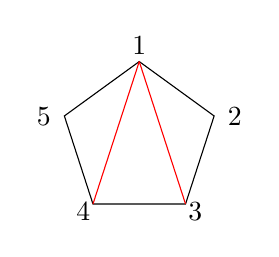
\begin{tikzpicture}
  \drawLabeledPentagon
  \draw[color=red] (P1) -- (P3);
  \draw[color=red] (P1) -- (P4);
\end{tikzpicture}
\end{equation}
We can immediately see the parallels with our $\Gr(2,5)$ situation (this is an example of the more general Pl\"ucker embedding which connects $\Gr(k,n)$ with projective space). Here we associate lines connecting points $i$ and $j$ with the Pl\"ucker coordinate $\ket{ij}$, and we see that the triangulations of the pentagon all describe points in $\Gr^+(2,5)$. In fact this correspondence holds between $n$-gons and $\Gr^+(2,n)$. 

A simple observation, but one at the very heart of cluster algebras, is that given some triangulation of a polygon one can create a \emph{new} triangulation by picking a quadrilateral and flipping its diagonal. For example:
\begin{equation}
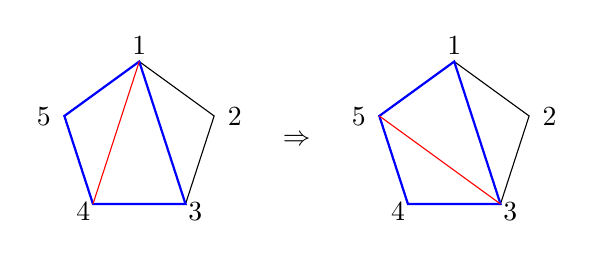
\begin{tikzpicture}
  \drawLabeledPentagon
  \draw[color=blue, thick] (P1) -- (P3) -- (P4) -- (P5) -- cycle;
  \draw[color=red] (P1) -- (P4);
  \draw (2,0) node {$\Rightarrow$};
\begin{scope}[xshift = 4cm]
  \drawLabeledPentagon
  \draw[color=blue, thick] (P1) -- (P3) -- (P4) -- (P5) -- cycle;
  \draw[color=red] (P5) -- (P3);
\end{scope}
\end{tikzpicture} 
\end{equation}
By repeatedly performing these flips one can generate all possible triangulations of a polygon:
\pagebreak
\begin{figure}[h!]
  \centering
  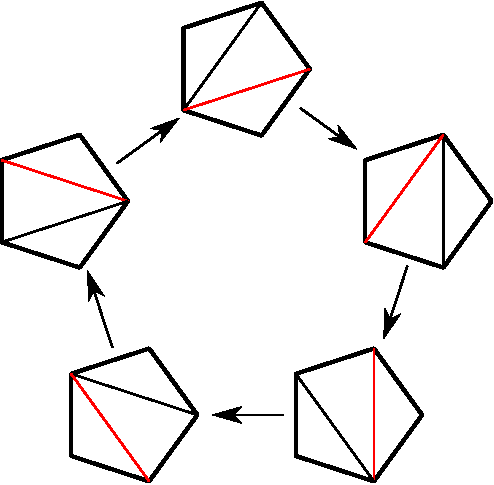
\includegraphics[scale=0.6]{pentagon-triangulations}
\end{figure}

\noindent where in each case the red diagonal gets flipped. 

Cluster algebras are a combinatorial tool which captures all of this structure (and much more!). The basic idea is that a cluser algebra is a collection of \emph{clusters}, which in this case represent individual triangulations of an $n$-gon, and these clusters are connected via a process called \emph{mutation}, which in this case is the flipping-the-diagonal process. \draftnote{more description of math applications of clsuter algebras? seiberg duality?}

\subsubsection*{Basic definition}

We'll begin by working through the cluster algebra for $\Gr(2,5)$. Each cluster is labeled by a collection of coordinates, which in this case are the edges of the pentagon along with the diagonals of the particular triangulation. These coordinates are then connected via an orientation of the pentagon and all subtriangles, for example:
\begin{equation}\label{eq:oriented-pentagon}
\begin{gathered}
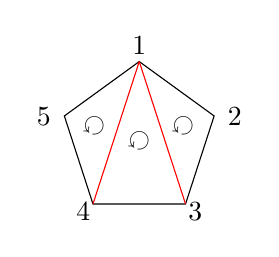
\begin{tikzpicture}
  \drawLabeledPentagon
  \draw[color=red] (P1) -- (P3);
  \draw[color=red] (P1) -- (P4);
  \draw (18:.6) node[rotate=144] {$\circlearrowleft$};
  \draw (0:0) node[rotate=144] {$\circlearrowleft$};
  \draw (162:.6) node[rotate=144] {$\circlearrowleft$};
\end{tikzpicture} 
\end{gathered}
\end{equation}
We can redraw this diagram as
\begin{equation}\label{eq:gr25-seed}
\begin{gathered}
\begin{xy} 0;<1pt,0pt>:<0pt,-1pt>::
	(25,25) *+{\langle 13\rangle} ="0",
	(75,25) *+{\langle 14\rangle} ="1",
	(125,25) *+{\framebox[5ex]{$\langle 15\rangle$}} ="2",
	(125,75) *+{\framebox[5ex]{$\langle 45\rangle$}} ="3",
	(75,75) *+{\framebox[5ex]{$\langle 34\rangle$}} ="4",
	(25,75) *+{\framebox[5ex]{$\langle 23\rangle$}} ="5",
	(0,0) *+{\framebox[5ex]{$\langle 12\rangle$}} ="6",
	(145,75) *+{},
	"0", {\ar"1"},
	"4", {\ar"0"},
	"0", {\ar"5"},
	"6", {\ar"0"},
	"1", {\ar"2"},
	"3", {\ar"1"},
	"1", {\ar"4"},
\end{xy}
\end{gathered}
\end{equation}
In this quiver diagram, we have an arrow between two Pl\"uckers $\ket{ab} \to \ket{cd}$ if the triangle orientations in eq. (\ref{eq:oriented-pentagon}) have segment $(ab)$ flowing into segment $(cd)$. The boxes around the $\ket{ii+1}$ indicate that they are \emph{frozen} -- in other words, we never change the outer edges of the pentagon, only the diagonal elements. The variables living at the frozen nodes can be thought of as parameterizing the boundary of our space, and the mutable nodes represent parameterizations of the interior. And lastly it is unnecessary to draw the arrows connecting the outer edges, as that is redundant (and unchanging) information. 

We have now drawn our first cluster (also sometimes called a seed). To review/introduce some terminology, the Pl\"uckers are called cluster $\a$-coordinates (sometimes also $\a$-variables), and they come in two flavors: mutable ($\ket{13}$ and $\ket{14}$) and frozen ($\ket{ii+1}$). The information of the arrows can be represented in terms of a skew-symmetric adjacency matrix
\begin{equation}
	b_{i j} = (\# \text{arrows}\; i \to j) - (\# \text{arrows}\; j \to i).
\label{eq:bijdef}
\end{equation}

The process of mutation, which we described geometrically in terms of flipping the diagonal, has a simple interpretation at the level of this quiver. In particular, given a quiver such as eq. (\ref{eq:gr25-seed}), chose a node $k$ with associated $\a$-coordinate $a_k$ to mutate on (this is equivalent to picking which diagonal to flip). Then draw a new quiver that changes $a_{k}$ to $a_{k}'$ defined by
\begin{equation}
  \label{eq:a-coord-mutation}
  a_{k} a_{k}' = \prod_{i \vert b_{i k} > 0} a_{i}^{b_{i k}} + \prod_{i \vert b_{i k} < 0} a_{i}^{-b_{i k}},
\end{equation} (with the understanding that an empty product is set to one) and leaves the other cluster coordinates unchanged. The arrows connecting the nodes in this new cluster are modified from the original cluster according to
\begin{itemize}
	\item for each path $i\to j \to k$, add an arrow $i\to j$,
	\item reverse all arrows on the edges incident with $k$,
	\item and remove any two-cycles that may have formed.
\end{itemize}
This creates a new adjacency matrix $b_{ij}'$ via 
\begin{equation}
  \label{eq:b-mutation}
  b'_{i j} =
  \begin{cases}
    -b_{i j}, &\quad \text{if $k \in \lbrace i, j\rbrace$,}\\
    b_{i j}, &\quad \text{if $b_{i k} b_{k j} \leq 0$,}\\
    b_{i j} + b_{i k} b_{k j}, &\quad \text{if $b_{i k}, b_{k j} > 0$,}\\
    b_{i j} - b_{i k} b_{k j}, &\quad \text{if $b_{i k}, b_{k j} < 0$.}
  \end{cases}
\end{equation}
Mutation is an involution, so mutating on $a_k'$ will take you back to the original cluster (as flipping the same diagonal twice will take you back to where you started). 

For our purposes, \emph{a cluster algebra is a set of quivers closed under mutation}. This means that mutating on any node of any quiver will generate a different quiver in the cluster algebra. The general procedure is to start with a quiver such as eq. (\ref{eq:gr25-seed}), with some collection of frozen and unfrozen nodes in a connected quiver, and continue mutating on all available nodes until you either close your set or convince yourself that the cluster algebra is infinite. 

We will end this brief introduction with a last piece of notation: cluster algebras are often referred to by particularly nice quiver types formed by their mutable nodes at some cluster. In the case of $\Gr(2,5)$, the mutable nodes of eq.~(\ref{eq:gr25-seed}) form an oriented $A_2$ Dynkin diagram, $\ket{13}\to\ket{14}$, and so we will often speak interchangeably of the cluster algebras for $\Gr(2,5)$ and $A_2$. This is a slight abuse of notation as the $\Gr(2,5)$ cluster algebra corresponds specifically to the cluster algebra generated by the collection of frozen and mutable nodes in eq.~(\ref{eq:gr25-seed}), whereas an $A_2$ cluster algebra is $a_1 \to a_2$ dressed with any (non-zero) number of frozen nodes. We will see how this language can be useful in the next section.

\subsection{Cluster \texorpdfstring{$\mathcal{X}$}{X}-coordinates}

Another important set of information encoded in cluster algebras are called Fock-Goncharov or $\x$-coordinates and were introduced in~\cite{FG03b}. As we will see in future sections, cluster \xcoords play a crucial role in connecting cluster algebras to polylogarithms and scattering amplitudes. While everything can be (and often is) phrased purely in terms of \acoords, we believe that emphasizing \xcoords allows for more direct connection with the full cluster algebraic structure. 

Given a quiver described by the matrix $b$, the $\a$- and $\x$-coordinates are related as follows:
\begin{equation}
	x_i = \prod_j a_j^{b_{ij}}. 	
\end{equation} 
For example, the quiver in eq.~(\ref{eq:gr25-seed}) has $\x$-coordinates 
\begin{equation}\label{def:xcoordsA2}
	\x_1 = \frac{\ket{12}\ket{34}}{\ket{14}\ket{23}}, \quad \x_2 = \frac{\ket{13}\ket{45}}{\ket{15}\ket{34}}.
\end{equation}
In the pentagon-triangulation picture, these $\x$-coordinates describe overlapping quadrilaterals:
\begin{equation}
\begin{gathered}
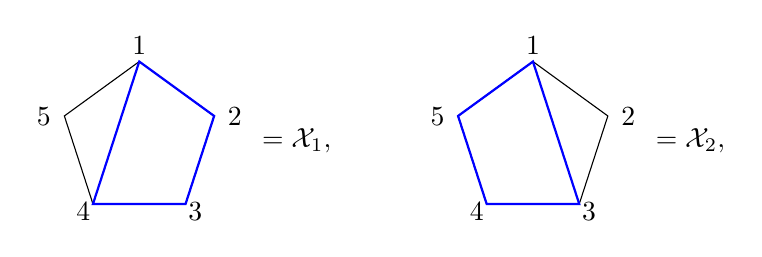
\begin{tikzpicture}
  \drawLabeledPentagon
  \draw[color=blue, thick] (P1) -- (P2) -- (P3) -- (P4) -- cycle;
  \draw (2,0) node {$=\x_1,$};
\begin{scope}[xshift = 5cm]
  \drawLabeledPentagon
  \draw[color=blue, thick] (P1) -- (P3) -- (P4) -- (P5) -- cycle;
  \draw (2,0) node {$=\x_2,$};
\end{scope}
\end{tikzpicture} 
\end{gathered}
\end{equation}
The mutation rules for the $\x$-coordinates are
\begin{equation}
  \label{eq:x-coord-mutation}
  x_{i}' =
  \begin{cases}
    x_{k}^{-1}, &\quad i=k,\\
    x_{i} (1+x_{k}^{\sgn b_{i k}})^{b_{i k}}, &\quad i \neq k
  \end{cases},
\end{equation}
For many applications in the rest of this work we will refer to cluster by their $\x$-coordinates alone, for example in this language we take the generic $A_2$ cluster algebra seed as 
\begin{equation}
	x_1 \to x_2.
\end{equation}
This again is a slight abuse of notation, in that it can be unclear, given a quiver, if one should use the \acoord mutation rules (\ref{eq:a-coord-mutation}) or \xcoord rules (\ref{eq:x-coord-mutation}). This ambiguity will be resolved in this work by that convention that if a quiver is given with no frozen nodes then it is referring to a collection of \xcoords. 

By continuing to mutate on alternating nodes (denoted below by \mbox{\color{red}{red}}) we generate the following sequence of clusters:
\begin{align}
  x_1 &\to \color{red}{x_2} \nl
  \color{red}{x_1(1+x_2)} &\leftarrow \frac{1}{x_2} \nl
  \frac{1}{x_1(1+x_2)} &\to \color{red}{\frac{x_2}{1+x_1+x_1 x_2}} \\
  \color{red}{\frac{x_1 x_2}{1+x_1}} &\leftarrow \frac{1+x_1+x_1 x_2}{x_2} \nl
  \frac{1+x_1}{x_1 x_2} &\to \color{red}{\frac{1}{x_1}} \nl
  \color{red}{x_2} &\leftarrow x_1 \nl
  &\vdots \nn
\end{align}
where the series then repeats. Note that by labeling the $\x$-coordinates as
\begin{equation}\label{def:a2-xcoords}
  \x_1 = 1/x_1, \quad \x_2 = x_2, \quad \x_3 = x_1(1+x_2), \quad 
  \x_4 = \frac{1+x_1+x_1 x_2}{x_2}, \quad \x_5 = \frac{1+x_1}{x_1 x_2},
\end{equation}
then the general mutation rule of eq. (\ref{eq:x-coord-mutation}) takes the simple form of
\begin{equation}\label{eq:exchange-relation}
  1+\x_i = \x_{i-1}\x_{i+1}.
\end{equation}
Putting this all together, we will generically refer to an $A_2$ cluster algebra as any set of clusters $1/\x_{i-1} \to \x_i$ for $i=1\ldots5$ where the $\x_i$ satisfy eq. (\ref{eq:exchange-relation}). We believe it is useful at this point to emphasize that one can take as input any $\{x_1, x_2\}$ and generate an associated $A_2$. For example, one could start with the quiver $3\to\frac{7}{2}$ and generate the $A_2$
\begin{equation}
\begin{gathered}
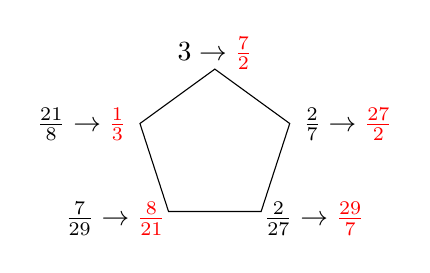
\begin{tikzpicture}
  \drawPentagon
  \draw (0,1.2) node {$3\to\color{red}{\frac{7}{2}}$};
  \draw (1,.3) node[anchor=west] {$\frac{2}{7} \to \color{red}{\frac{27}{2}} $};
  \draw (.5,-.9) node[anchor=west] {$\frac{2}{27} \to \color{red}{\frac{29}{7}}$};
  \draw (-.5,-.9) node[anchor=east] {$\frac{7}{29} \to \color{red}{\frac{8}{21}}$};
  \draw (-1,.3) node[anchor=east] {$\frac{21}{8} \to \color{red}{\frac{1}{3}}$};
\end{tikzpicture}
\end{gathered}.
\end{equation}
(Mutating on the node in red moves you clockwise around the pentagon.) In future sections it will be necessary to consider collections of multiple $A_2$ algebras, in such cases we label them by only one of their clusters, e.g. $x_1 \to x_2$, with the understanding that we are referring to the $A_2$ which contains that cluster as an element.

\draftnote{poisson bracket?}

\subsection{Subalgebras}\label{sec:subalgebras}

Cluster algebras contain a rich and intricate subalgebra structure which will be critical for our upcoming physics applications. We can study a simple example by looking at triangulations of a hexagon, which is equivalently described by the cluster algebra associated with $\Gr(2,6)$:
\begin{equation}\label{eq:gr26-seed}
\begin{gathered}
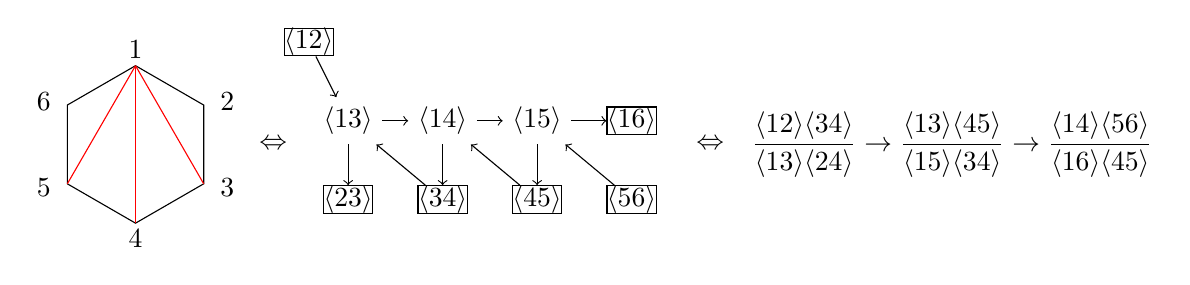
\begin{tikzpicture}
	\drawLabeledHexagon
  	\draw[color=red] (P1) -- (P3);
  	\draw[color=red] (P1) -- (P4);
  	\draw[color=red] (P1) -- (P5);
	\draw (1.75,0) node {$\Leftrightarrow$};
	\begin{scope}[xshift = .2cm, yshift = .3cm]
	\def \xSep {1.2}
	\def \xInit {2.5}
    \node (13) at (\xInit,0) {$\ket{13}$};
    \node (14) at (\xInit+\xSep,0) {$\ket{14}$};
    \node (15) at (\xInit+2*\xSep,0) {$\ket{15}$};
	\node[draw, inner sep=0mm] (12) at (2,1) {$\ket{12}$};
    \node[draw, inner sep=0mm] (16) at (\xInit+3*\xSep,0) {$\ket{16}$};
    \node[draw, inner sep=0mm] (56) at (\xInit+3*\xSep,-1) {$\ket{56}$};
    \node[draw, inner sep=0mm] (45) at (\xInit+2*\xSep,-1) {$\ket{45}$};
    \node[draw, inner sep=0mm] (34) at (\xInit+\xSep,-1) {$\ket{34}$};
    \node[draw, inner sep=0mm] (23) at (\xInit,-1) {$\ket{23}$};
    \draw[->] (12) -- (13);
    \draw[->] (13) -- (14);
    \draw[->] (14) -- (15);
    \draw[->] (15) -- (16);
    \draw[->] (13) -- (23);
    \draw[->] (34) -- (13);
    \draw[->] (14) -- (34);
    \draw[->] (45) -- (14);
    \draw[->] (15) -- (45);
    \draw[->] (56) -- (15);
    \end{scope}
    \draw (7.3,0) node {$\Leftrightarrow$};
    \node[anchor=west] at (7.7,0) {$\displaystyle \frac{\ket{12}\ket{34}}{\ket{13}\ket{24}}\to\frac{\ket{13}\ket{45}}{\ket{15}\ket{34}}\to\frac{\ket{14}\ket{56}}{\ket{16}\ket{45}} $};
\end{tikzpicture} 
\end{gathered}
\end{equation}
Here we have given the seed cluster for $\Gr(2,6)$ in the triangulation, \acoord, and \xcoord representations, respectively. Since the mutable nodes take the form of an $A_3$ Dynkin diagram, we often speak of $\Gr(2,6)$ and $A_3$ interchangeably, just as we did with $\Gr(2,5) \simeq A_2$. 

The $\Gr(2,6)$ cluster algebra features 14 clusters, and these clusters can be grouped together in to multiple (overlapping) sets which constitute subalgebras. A simple example is the collection of all triangulations which involve the cord $\ket{15}$. It is easy to see that this set contains 5 clusters and is itself a cluster algebra generated via mutations by taking eq.~(\ref{eq:gr26-seed}), ``freezing'' the cord $\ket{15}$, then mutating on the other two cluster coordinates (in the \xcoord language, this is equivalent to only mutating on the left and middle nodes of eq.~(\ref{eq:gr26-seed})). This of course is the cluster algebra of triangulating the pentagon formed by points $1,\ldots,5$:
\begin{equation}
\begin{gathered}
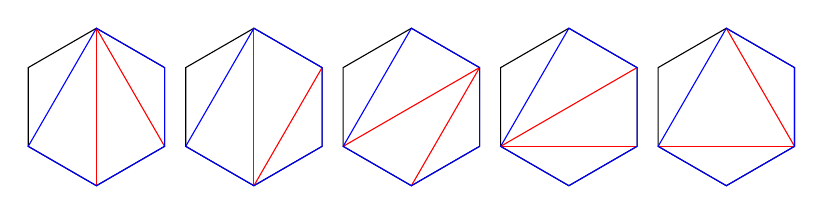
\begin{tikzpicture}
	\drawHexagon
  	\draw[color=red] (P1) -- (P3);
  	\draw[color=red] (P1) -- (P4);
	\draw[color=blue] (P1) -- (P2) -- (P3) -- (P4) -- (P5) -- cycle;
	\begin{scope}[xshift=2cm]
	\drawHexagon
  	\draw[color=red] (P2) -- (P4);
  	\draw[color=red] (P1) -- (P4);
	\draw[color=blue] (P1) -- (P2) -- (P3) -- (P4) -- (P5) -- cycle;
	\end{scope}
	\begin{scope}[xshift=4cm]
	\drawHexagon
  	\draw[color=red] (P2) -- (P4);
  	\draw[color=red] (P2) -- (P5);
	\draw[color=blue] (P1) -- (P2) -- (P3) -- (P4) -- (P5) -- cycle;
	\end{scope}
	\begin{scope}[xshift=6cm]
	\drawHexagon
  	\draw[color=red] (P2) -- (P5);
  	\draw[color=red] (P3) -- (P5);
	\draw[color=blue] (P1) -- (P2) -- (P3) -- (P4) -- (P5) -- cycle;
	\end{scope}
	\begin{scope}[xshift=8cm]
	\drawHexagon
  	\draw[color=red] (P1) -- (P3);
  	\draw[color=red] (P3) -- (P5);
	\draw[color=blue] (P1) -- (P2) -- (P3) -- (P4) -- (P5) -- cycle;
	\end{scope}
\end{tikzpicture}
\end{gathered}.
\end{equation}
In practice, we refer to the collection of clusters that share this pentagon as an $A_2$ subalgebra of $\Gr(2,6)$. Instead of freezing the cord $\ket{15}$ we could have frozen the cord $\ket{14}$, in which case we generate an $A_1 \times A_1$ subalgebra, as $A_1$ corresponds to the triangulations of a square and the cord $\ket{14}$ divides the hexagon in to two non-overlapping squares:
\begin{equation}
\begin{gathered}
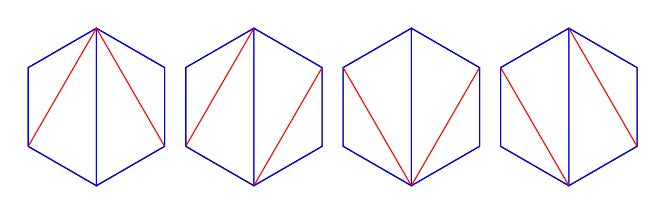
\begin{tikzpicture}
	\drawHexagon
  	\draw[color=blue] (P1) -- (P2) -- (P3) -- (P4) -- cycle;
  	\draw[color=blue] (P1) -- (P4) -- (P5) -- (P6) -- cycle;
  	\draw[color=red] (P1) -- (P5);
  	\draw[color=red] (P1) -- (P3);
  	\begin{scope}[xshift=2cm]
	\drawHexagon
  	\draw[color=blue] (P1) -- (P2) -- (P3) -- (P4) -- cycle;
  	\draw[color=blue] (P1) -- (P4) -- (P5) -- (P6) -- cycle;
  	\draw[color=red] (P1) -- (P5);
  	\draw[color=red] (P4) -- (P2);
	\end{scope}
	\begin{scope}[xshift=4cm]
	\drawHexagon
  	\draw[color=blue] (P1) -- (P2) -- (P3) -- (P4) -- cycle;
  	\draw[color=blue] (P1) -- (P4) -- (P5) -- (P6) -- cycle;
  	\draw[color=red] (P6) -- (P4);
  	\draw[color=red] (P4) -- (P2);
	\end{scope}
	\begin{scope}[xshift=6cm]
	\drawHexagon
  	\draw[color=blue] (P1) -- (P2) -- (P3) -- (P4) -- cycle;
  	\draw[color=blue] (P1) -- (P4) -- (P5) -- (P6) -- cycle;
  	\draw[color=red] (P6) -- (P4);
  	\draw[color=red] (P1) -- (P3);
	\end{scope}
\end{tikzpicture}
\end{gathered}.
\end{equation}
Larger cluster algebras contain many subalgebras of different types. We have catalogued the counting of these subalgebras for many relevant cluster algebras in Appendix~\ref{appendix:subalgebras}.


\subsection{Associahedra}

The mutation paths between clusters, and which sets of clusters group together to form subalgebras, can be easily visualized through an object known as the associahedron (also called the Stasheff polytope) for a given cluster algebra. This polytope is formed by vertices representing an indivual cluster, and edges are drawn between clusters connected via mutation. So the figure\\

\begin{figure}[h!]
  \centering
  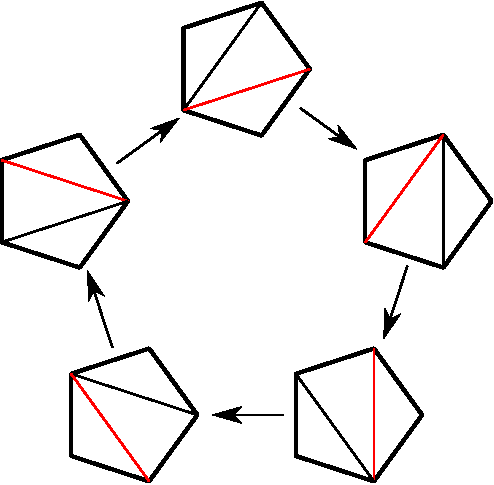
\includegraphics[scale=0.6]{pentagon-triangulations}
\end{figure}
\noindent \draftnote{create new version} is in fact the $\Gr(2,5)$ or $A_2$ associahedron, coincidentally takes the form of a pentagon. 

The associahedron associated with the $\Gr(2,6) \leftrightarrow A_3$ cluster algebra (i.e. triangulations of a hexagon) is\\

\begin{figure}[h!]\label{fig:a3-poly}
  \centering
  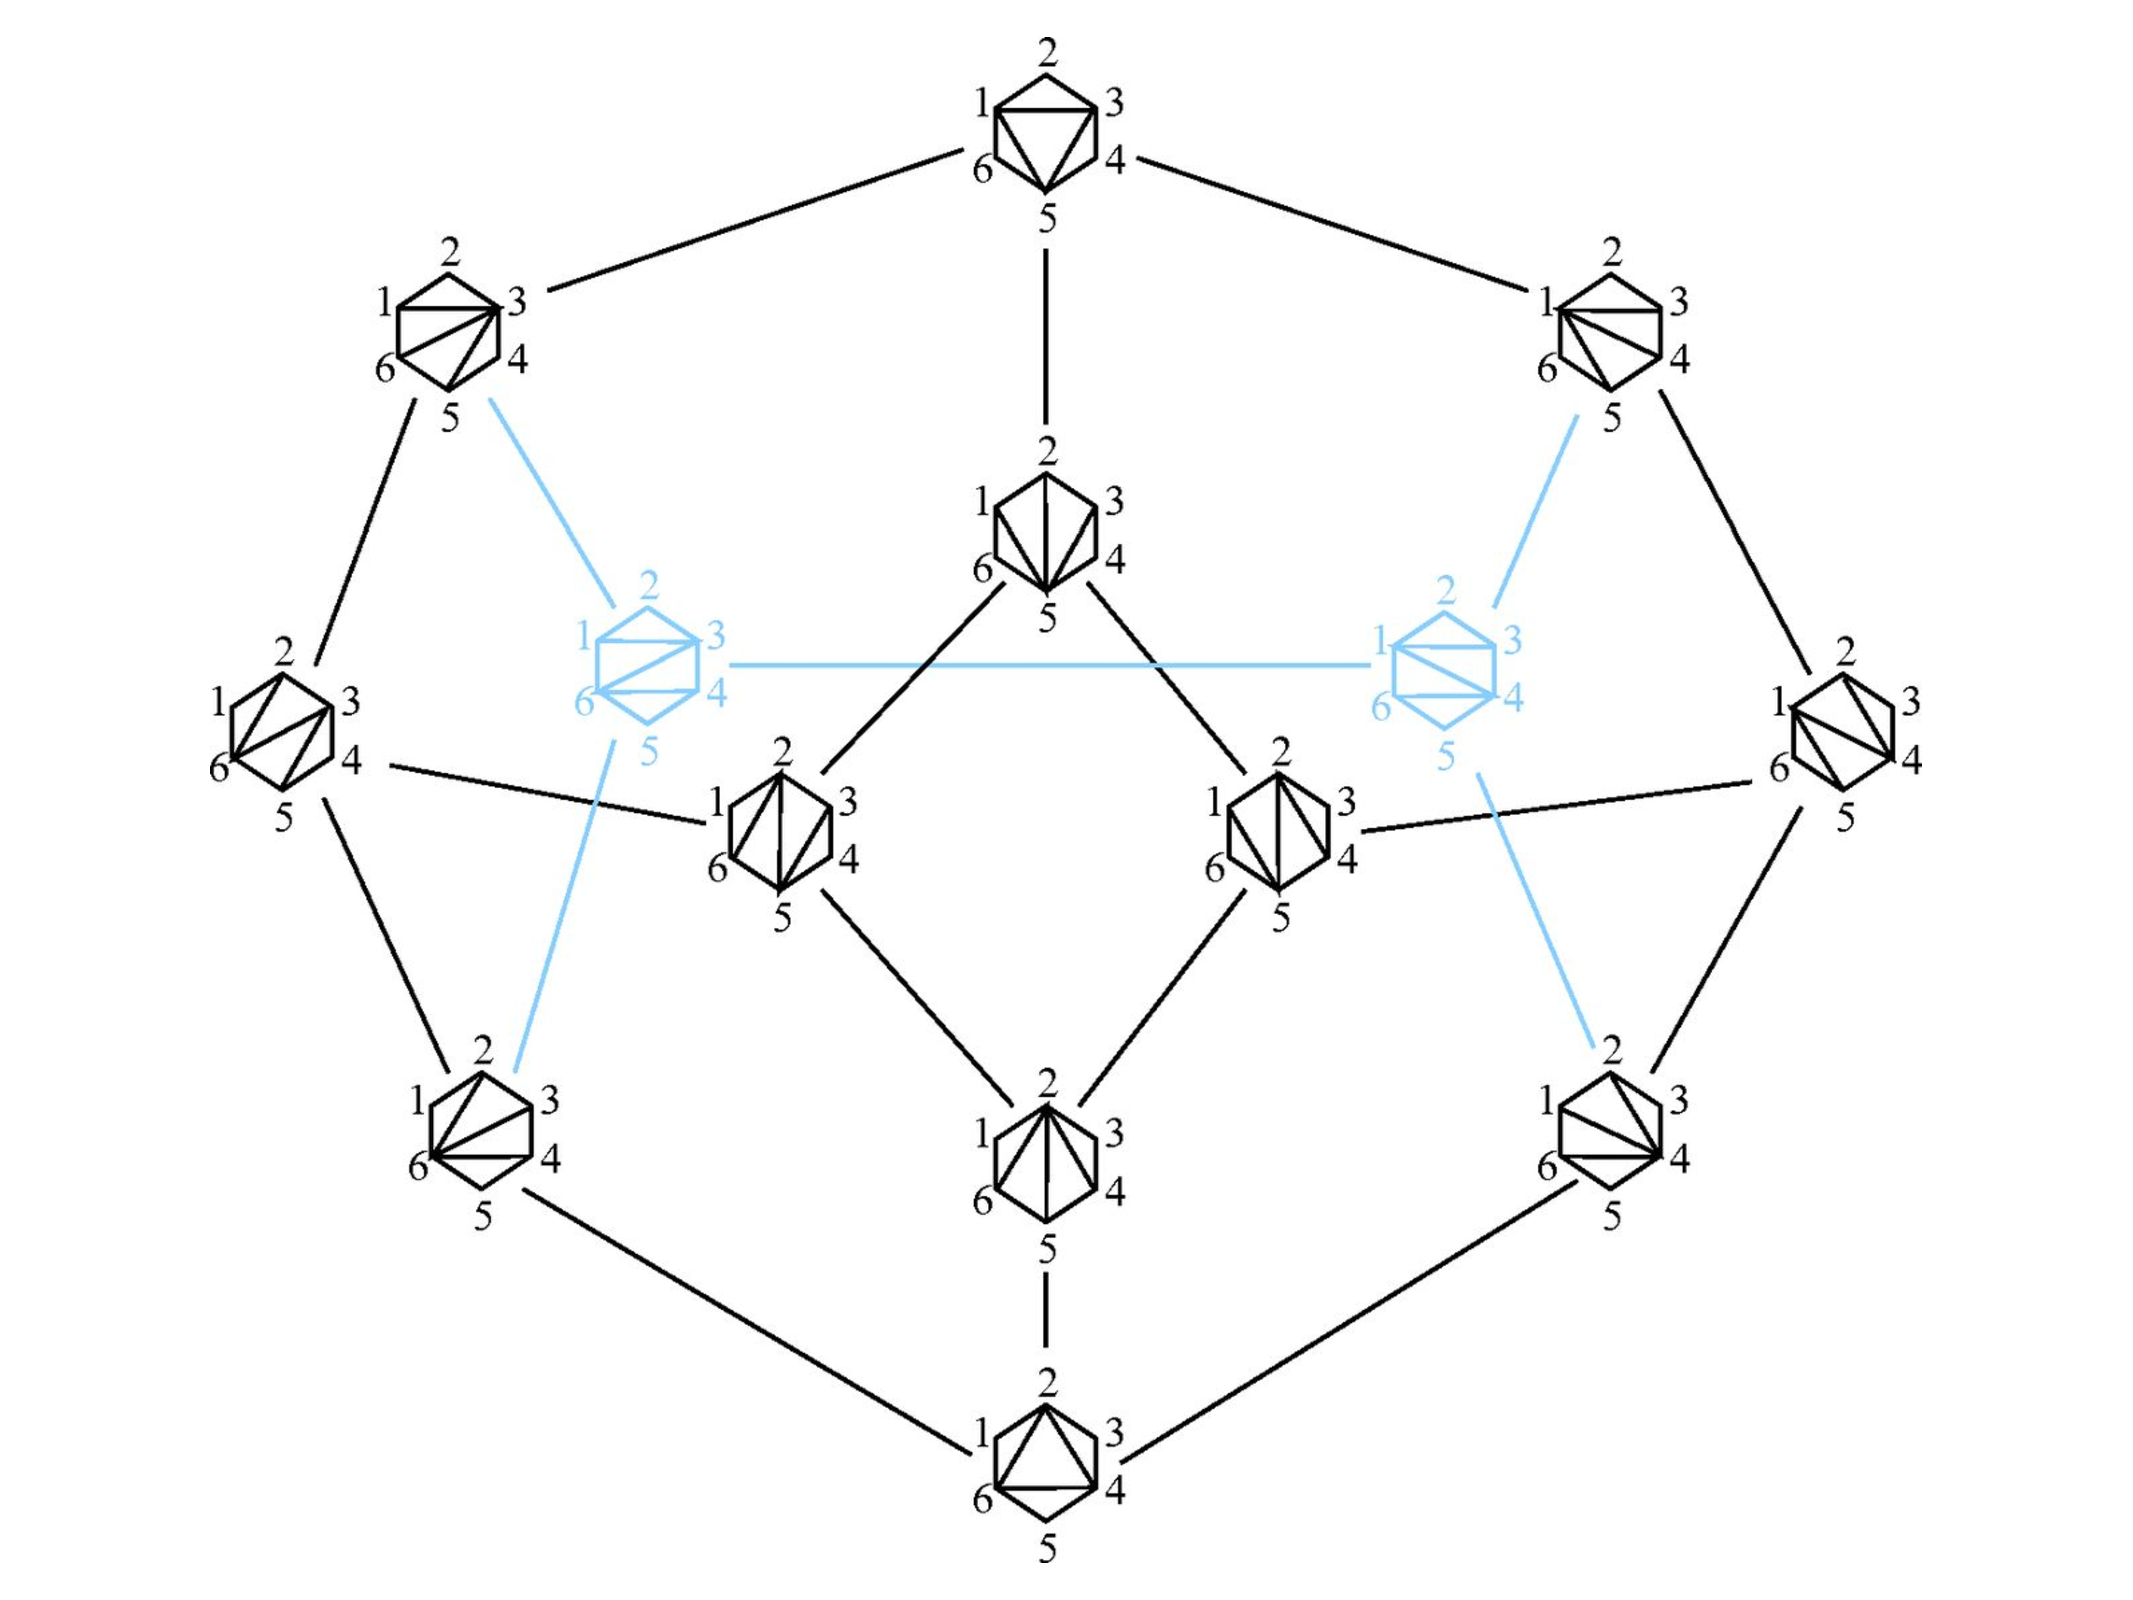
\includegraphics[scale=0.25]{a3-associahedron}
  \caption{The associahedron for $A_3\simeq\Gr(2,6)$.}
\end{figure}

\noindent \draftnote{create new version} This associahedron has 14 vertices, corresponding to the 14 clusters, with 3 square faces and 6 pentagonal faces. The square faces represent $A_1\times A_1$ subalgebras, and the pentagonal faces are $A_2$ subalgebras as discussed in the previous section. Because of the Grassmannian duality $\Gr(2,6) \simeq \Gr(4,6)$, this (remarkably simple!) cluster algebra and associahedron play an integral role in the momentum twistors for 6-particle kinematics for $\mathcal{N}=4$ SYM. 

Associahedra for larger cluster algebras can become quite complicated, with intricate subpolytope/subalgebra structures. For example, the associahedron for $\Gr(4,7)\simeq E_6$, which will be the focus of much of the rest of this paper, is

\begin{figure}[h!]\label{fig:e6-poly}
  \centering
  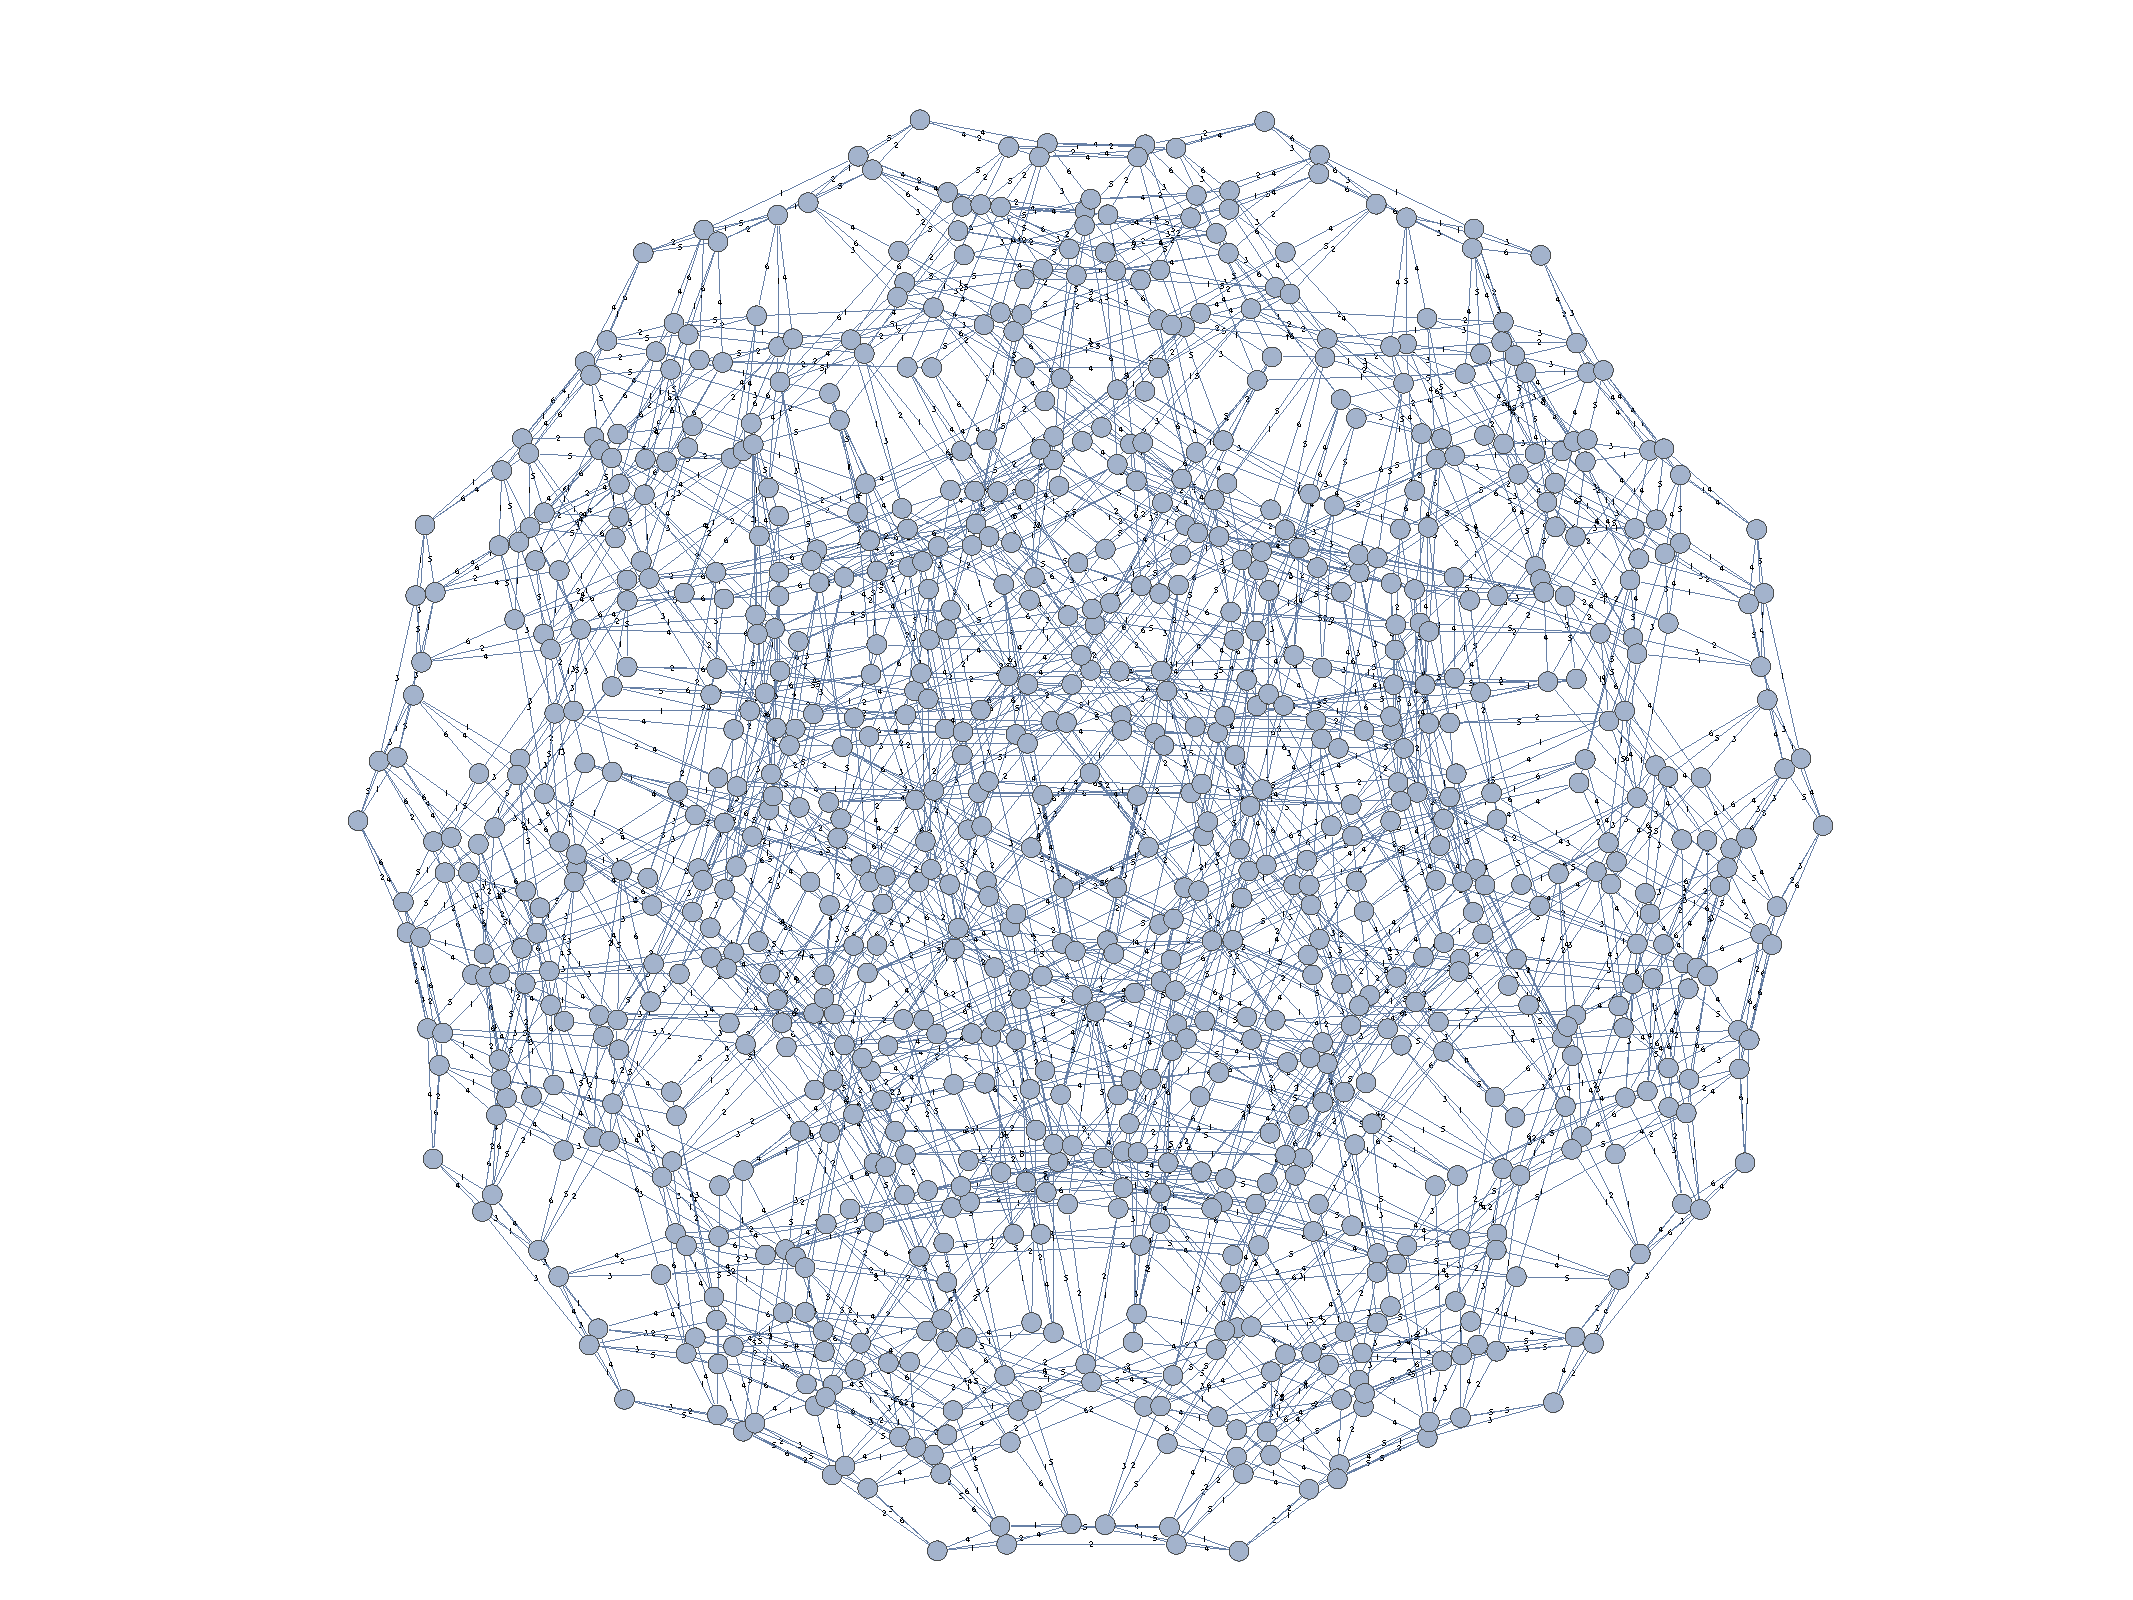
\includegraphics[scale=0.25]{e6-associahedron}
  \caption{The associahedron for $E_6\simeq\Gr(4,7)$.}
\end{figure}
\noindent It features 833 clusters/vertices of valence 6. The dimension-2 faces are 1785 squares and 1071 pentagons, and there are 49 different $A$-coordinates that appear. 

\subsection{Grassmannian cluster algebras}

So far we have leaned heavily on the correspondence between triangulations of an $n$-gon and the cluster algebra for $\Gr(2,n)$. Based on the examples of $\Gr(2,5)$ and $\Gr(2,6)$, it is not hard to write down a generic seed cluster for $\Gr(2,n)$ based off the triangulation of all cords $\ket{13},\ldots,\ket{1n{-}1}$:
\begin{equation}\label{eq:g2n-seed}
\begin{gathered}
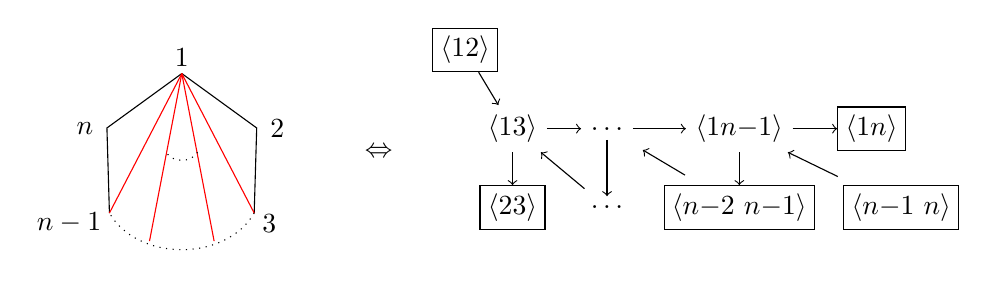
\begin{tikzpicture}
	\coordinate (P1) at (90:1);
	\coordinate (P2) at (18:1);
	\coordinate (P3) at (320:1.2);
	\coordinate (P4) at (220:1.2);
	\coordinate (P5) at (162:1);
	\draw (0,1.2) node {1};
	\draw (1,.3) node[anchor=west] {2};
	\draw (.9,-.9) node[anchor=west] {3};
	\draw (-.9,-.9) node[anchor=east] {$n-1$};
	\draw (-1,.3) node[anchor=east] {$n$};
	\draw (P1) -- (P2) -- (P3);
	\draw[dotted] (P3) to[out=240,in=300] (P4);
	\draw (P4) -- (P5) -- (P1);
	\draw[red] (P1) -- (P3);
	\draw[red] (P1) -- (P4);
	\draw[red] (P1) -- (290:1.2);
	\draw[red] (P1) -- (250:1.2);
	\draw[dotted] (.2,0) to[out=240,in=300] (-.2,0);
	\draw (2.5,0) node {$\Leftrightarrow$};
	\begin{scope}[xshift = .2cm, yshift = .3cm]
	\def \xSep {1.2}
	\def \xInit {4}
    \node (13) at (\xInit,0) {$\ket{13}$};
    \node (14) at (\xInit+\xSep,0) {$\ldots$};
    \node (15) at (\xInit+2.4*\xSep,0) {$\ket{1n{-}1}$};
	\node[draw, inner sep=1mm] (12) at (\xInit-.5*\xSep,1) {$\ket{12}$};
    \node[draw, inner sep=1mm] (16) at (\xInit+3.8*\xSep,0) {$\ket{1n}$};
    \node[draw, inner sep=1mm,anchor=west] (56) at (\xInit+3.5*\xSep,-1) {$\ket{n{-}1~n}$};
    \node[draw, inner sep=1mm] (45) at (\xInit+2.4*\xSep,-1) {$\ket{n{-}2~n{-}1}$};
    \node (34) at (\xInit+\xSep,-1) {$\ldots$};
    \node[draw, inner sep=1mm] (23) at (\xInit,-1) {$\ket{23}$};
    \draw[->] (12) -- (13);
    \draw[->] (13) -- (14);
    \draw[->] (14) -- (15);
    \draw[->] (15) -- (16);
    \draw[->] (13) -- (23);
    \draw[->, shorten <= 0.15cm] (34) -- (13);
    \draw[->] (14) -- (34);
    \draw[->, shorten <= 0.25cm, shorten >= 0.25cm] (45) -- (14);
    \draw[->] (15) -- (45);
    \draw[->, shorten <= 0.25cm] (56) -- (15);
    \end{scope}
\end{tikzpicture}
\end{gathered}.
\end{equation}
Here one sees that the mutable nodes for $\Gr(k,n)$ always can take the form of an $A_{n-3}$ Dynkin diagram. 

For $\Gr(k>2,n)$, there is no longer a simple connection with triangulations or Dynkin diagrams. However, as shown by Scott \cite{1088.22009} there exists a generalization of eq.~(\ref{eq:g2n-seed}) valid for all $k,n$:
\begin{equation}\label{eq:gkn-seed}
\begin{gathered}
\begin{xy} 0;<-.5pt,0pt>:<0pt,-.5pt>::
	(-100,0) *+{\framebox[10ex]{$\ket{1,\ldots,k}$}} ="-1",
	(0,0) *+{f_{1l}} ="0",
	(75,0) *+{\cdots} ="1",
	(150,0) *+{f_{13}} ="2",
	(225,0) *+{f_{12}} ="3",
	(300,0) *+{\framebox[5ex]{$f_{11}$}} ="4",
	(0,75) *+{f_{2l}} ="5",
	(75,75) *+{\cdots} ="6",
	(150,75) *+{f_{23}} ="7",
	(225,75) *+{f_{22}} ="8",
	(300,75) *+{\framebox[5ex]{$f_{21}$}} ="9",
	(0,150) *+{\vdots} ="10",
	(75,150) *+{\vdots} ="11",
	(150,150) *+{\vdots} ="12",
	(225,150) *+{\vdots} ="13",
	(300,150) *+{\vdots} ="14",
	(0,225) *+{\framebox[5ex]{$f_{kl}$}} ="15",
	(75,225) *+{\cdots} ="16",
	(150,225) *+{\framebox[5ex]{$f_{k3}$}} ="17",
	(225,225) *+{\framebox[5ex]{$f_{k2}$}} ="18",
	(300,225) *+{\framebox[5ex]{$f_{k1}$}} ="19",
	(-60,0) *+{} ="20",
	"0", {\ar"-1"},
	"1", {\ar"0"},
	"5", {\ar"0"},
	"0", {\ar"6"},
	"2", {\ar"1"},
	"3", {\ar"2"},
	"7", {\ar"2"},
	"2", {\ar"8"},
	"4", {\ar"3"},
	"8", {\ar"3"},
	"3", {\ar"9"},
	"6", {\ar"5"},
	"7", {\ar"6"},
	"8", {\ar"7"},
	"9", {\ar"8"},
	"7", {\ar"13"},
	"12", {\ar"7"},
	"13", {\ar"8"},
	"10", {\ar"5"},
	"14", {\ar"8"},
	"15", {\ar"10"},
	"17", {\ar"12"},
	"13", {\ar"19"},
	"12", {\ar"18"},
	"18", {\ar"13"},
\end{xy}
\end{gathered}
\end{equation}
where $l=n-k$ and 
\begin{equation}
  f_{i j} =
  \begin{cases}
    \langle i+1, \dotsc, k, k+j, \dotsc, i+j+k-1\rangle, \qquad &i \leq l-j+1,\\
    \langle 1, \dotsc, i+j-l-1, i+1, \dotsc, k, k+j, \dotsc, n\rangle, \qquad &i >l-j+1
  \end{cases}.
\end{equation}
(Note that evaluating the above expression at $k=2$ will give a cyclically rotated version of eq.~(\ref{eq:g2n-seed})). While the connection with triangulations is not applicable in general, the clusters generated from eq.~(\ref{eq:gkn-seed}) still give a coordinate chart for $\Gr^+(k,n)$ (though the coordinates won't always be simple Pl\"uckers, arbitrarily complicated polynomials of Pl\"uckers will appear as well). The cluster algebra for $\Gr(k,n)$ is therefore of rank $(n-k-1)(k-1)$, i.e. the number of mutable nodes in eq.~(\ref{eq:gkn-seed}). 

We have emphasized Grassmannian cluster algebras so far for two reasons: 1) the correspondence with triangulations and positive matrices make them easy to gain an intuition for and 2) the cluster algebra for $\Gr(4,n)$ is intimately connected to $n$-particle kinematics in $\mathcal{N}=4$ SYM. Let us now address point 2 a bit more in detail.


\subsubsection*{Applications to momentum twistors and \pdfeq{\mathcal{N}}=4 SYM}

An immediate connection between $\Gr(4,n)$ and $\mathcal{N}=4$ SYM is that the $\x$-coordinates are dual-conformal invariant cross-ratios and appear as arguments of relevant physical functions. We can see this for example in the two-loop, six-particle remainder function 
\begin{align}
	R^{(2)}_6 = &\sum_{\text{cyclic}} \text{Li}_4\left(-\frac{\langle 1234 \rangle \langle 2356 \rangle}{\langle 1236 \rangle \langle 2345 \rangle}\right) - \frac{1}{4} \text{Li}_4 \left(-\frac{\langle 1246 \rangle \langle 1345 \rangle}{\langle 1234 \rangle \langle 1456 \rangle}\right)\nl
	&+\text{products of } \text{Li}_{k}(-x) \text{ functions of lower weight}\\ &\quad~\text{with the same set of arguments.}\nn
\end{align}
\draftnote{more}

We will go in to much further detail on the connections between cluster algebras and $\mathcal{N}$=4 SYM in future sections. However, for now we will elaborate on the connections between cluster algebras and polylogarithms. For this we do not need to constrain ourselves to Grassmannian cluster algebras, and so for the next few sections we will work with the slightly more abstact language of quivers of generic \xcoords, i.e. $x_1 \to x_2$. 

\subsection{An overview of finite cluster algebras}\label{sec:finite-algebras}

One can, in principle, generate a cluster algebra by drawing any oriented quiver (even with weights), and then following the mutation rules for \acoords, eq.~(\ref{eq:a-coord-mutation}), if there are frozen nodes, or \xcoords, eq.~(\ref{eq:x-coord-mutation}), if not. However, generic quivers will produce very complicated cluster algebras -- in fact, for wide classes of seed quivers the the mutation rules generate infinite numbers of clusters, each with a distinct set of (infinitely complicated) coordinates. \footnote{There is a further distinction in the infinite case between cluster algebras which contain a finite number of quiver types (still with an infinite number of cluster coordinates), and those which contain infinitely many quivers as well as coordinates.} For the rest of this paper we will be concerned with finite algebras, and will leave discussion of the infinite cases to a companion publication \cite{}. 

Fortunately, Fomin and Zelevinksy classified all finite cluster algebras in \cite{1054.17024}. In particular, they showed that a cluster algebra is of finite type iff the mutable part of its quiver at some cluster takes the form of an oriented, simply-laced Dynkin diagram: $A_n, D_n, E_{n\le8}$. We will describe several of the relevant cases to give the reader a flavor for the world of finite algebras. 

As mentioned previously, cluster algebras of type $A_n$
\begin{equation}\label{def:An}
  x_1\to x_2\to \ldots \to x_n
\end{equation}
correspond to cluster algebras for $\Gr(2,n{+}3)$). Each cluster can be though as a triangulation of an $(n+3)$-gon, each \acoord is a cord, and each \xcoord is a quadrilateral with a cord as a diagonal embedded in the $(n+3)$-gon. This makes the counting easy: the number of clusters for $A_n$ is given by the Catalan number $C(n+1)$, the number of \acoords is $\binom{n+3}{2}-n$, and the number of \xcoords is $2\binom{n+3}{4}$. Subalgebras correspond to embedding a smaller polygon in to the $(n+3)$-gon, for example there are $56=\binom{8}{5}$ pentagonal embeddings in an octagon, and so there are 56 $A_2$ subalgebras in $A_5$. 

The cluster algebra $D_4$
\begin{equation}\label{def:D4}
    \begin{gathered}
    \begin{xy} 0;<1pt,0pt>:<0pt,-1pt>::
      (0,20) *+{x_1} ="1",
      (30,20) *+{x_2} ="2",
      (60,0) *+{x_3} ="3",
      (60,40) *+{x_4} ="4",
      "1", {\ar"2"},
      "2", {\ar"3"},
      "2", {\ar"4"},
    \end{xy}
    \end{gathered}
\end{equation}
turns out to be connected to $\Gr(3,6)$. It has 50 clusters, 16 \acoords, and 104 \xcoords. There are 36 $A_2$ subalgebras and 12 $A_3$ subalgebras. It is also a highly symmetric cluster algebra, as we will discuss in section~\ref{sec:automorphisms}.

The cluster algebra $D_5$
\begin{equation}\label{def:D5}
    \begin{gathered}
    \begin{xy} 0;<1pt,0pt>:<0pt,-1pt>::
      (0,20) *+{x_1} ="1",
      (30,20) *+{x_2} ="2",
      (60,20) *+{x_3} ="3",
      (90,0) *+{x_4} ="4",
      (90,40) *+{x_5} ="5",
      "1", {\ar"2"},
      "2", {\ar"3"},
      "3", {\ar"4"},
      "3", {\ar"5"},
    \end{xy}
    \end{gathered}
\end{equation}
is not immediately connected with any Grassmannian, although it appears as a subalgebra of any $\Gr(k,n)$ with rank $> 5$. $D_5$ has 182 clusters, 25 \acoords, and 260 \xcoords. There are 125 distinct $A_2$ subalgebras, 65 $A_3$, 10 $A_4$, and 5 $D_4$. 

Finally, we describe the cluster algebra $E_6$
\begin{equation}\label{def:E6}
    \begin{gathered}
    \begin{xy} 0;<1pt,0pt>:<0pt,-1pt>::
      (0,0) *+{x_1} ="1",
      (30,0) *+{x_2} ="2",
      (60,0) *+{x_3} ="3",
      (60,-25) *+{x_4} ="4",
      (90,0) *+{x_5} ="5",
      (120,0) *+{x_5} ="6",
      "1", {\ar"2"},
      "2", {\ar"3"},
      "3", {\ar"4"},
      "5", {\ar"3"},
      "6", {\ar"5"},
    \end{xy}
    \end{gathered}
\end{equation}
which is connected to $\Gr(4,7)$. The associahedron for this algebra is displayed in figure~\ref{fig:e6-poly}. The algebra hashas 833 clusters, 42 \acoords, and 770 \xcoords. The subalgebra counting is: 
\begin{equation}
\begin{tabular}{ c|c|c|c|c|c} 
 $A_2$ & $A_3$ & $A_4$ & $D_4$ & $A_5$ & $D_5$ \\ 
 \hline
504 & 364 & 98 & 35 & 7 & 14
\end{tabular}.
\end{equation}

For a more thorough tabulation of the subalgebra structure of these algebras, refer to appendix~\ref{appendix:subalgebras}.

\subsection{Cluster automorphisms}\label{sec:automorphisms}

See \cite{Chang:2015} for a more thorough mathematical introduction. The simplest example of a cluster automorphism is what we will call a direct automorphism. Let $\a$ be a cluster algebra. Then $f: \a \to \a$ is direct automorphism of $\a$ if
\begin{itemize}
  \item for every cluster $\mathbf{x}$ of $\a$, $f(\mathbf{x})$ is also a cluster of $\a$,
  \item $f$ respects mutations, i.e. $f(\mu(x_i,\mathbf{x})) = \mu(f(x_i),f(\mathbf{x}))$.
 \end{itemize} 
A simple example of this for $A_2$ is the map
\begin{equation}
  \sigma_{A_2}:\quad \mathcal{X}_i \to \mathcal{X}_{i+1},
\end{equation}
which cycles the five clusters $1/\x_i\to \x_{i+1}$ amongst themselves, and can be cast in terms of the seed variables $x_1, x_2$ as 
\begin{equation}
  \sigma_{A_2}:\quad x_1\to \frac{1}{x_2},~~ x_2\to x_1(1+x_2).
\end{equation}

A less obvious example of a cluster automorphism is what are called indirect automorphisms, which respect mutations but do not map clusters directly on to clusters; instead
\begin{itemize}
  \item for every cluster $\mathbf{x}$ of $\a$, $f(\mathbf{x})$ + invert all nodes + swap direction of all arrows\\ = a cluster of $\a$.
\end{itemize}
For $A_2$ we have the indirect automorphism
\begin{equation}
  \tau_{A_2}:\quad \mathcal{X}_i \to \mathcal{X}_{6-i},
\end{equation}
where indices are understood to be mod 5, and can instead be cast in terms of the seed variables $x_1, x_2$ as
\begin{equation}
  \tau_{A_2}:\quad x_1 \to \frac{1}{x_2}, ~~x_2 \to \frac{1}{x_1}.
\end{equation}
We can see how this works in a simple example
\begin{align}
  \tau_{A_2}(1/\x_1 \to \x_2) =&~1/\x_5 \to \x_4 \nl
  \Rightarrow &\text{ invert each node and swap direction of all arrows }\\ 
  =&~\x_5 \leftarrow 1/\x_4, \text{ which is in the original $A_2$}.\nn
\end{align}
It is useful to think of indirect automorphisms as generating a ``mirror'' or ``flipped'' version of the original $\a$, where the total collection of $\x$-coordinates is the same, but their Poisson bracket has flipped sign. The existence of this flip then can be seen as resulting from the choice of assigning $b_{ij}$ = (\# arrows $i\to j$) - (\# arrows $j \to i$), where instead we could have chosen $b_{ij}$ = (\# arrows $j \to i$) - (\# arrows $i\to j$) and still generated the same cluster algebraic structure, albeit with different labels for the nodes. In the generic case this is an arbitrary choice, and $\tau$ captures the superficiality of the notation change.

The automorphisms $\sigma_{A_2}$ and $\tau_{A_2}$ generate the complete automorphism group for $A_2$, namely, $D_5$ (the notation here is regretably redundant; here we are referring to the dihedral group of five elements, which is of course distinct from the Dynkin diagram $D_5$ -- we hope that context will clarify to the reader what we mean in each case). We now list generators for the automorphism groups of the finite algebras discussed already. First we adopt the notation
\begin{equation}
	x_{i_1,\ldots, i_k} = \sum_{a=1}^k \prod_{b=1}^a x_{i_b} = x_{i_1}+x_{i_1}x_{i_2} + \ldots + x_{i_1}\cdots x_{i_k}.
\end{equation}

Cluster algebras of type $A_n$, as defined in eq.~(\ref{def:An}), have automorphism group $D_{n+3}$, with a cyclic generator $\sigma_{A_n}$ (direct, length $n+3$)
\begin{equation}
  \sigma_{A_n}:\quad x_{k<n} \to \frac{x_{k+1}(1+x_{1,\ldots,k-1})}{1+x_{1,\ldots,k+1}},~~x_n\to\frac{1+x_{1,\ldots,n-1}}{\prod_{i=1}^n x_i}
\end{equation}
and flip generator $\tau_{A_n}$ (indirect)
\begin{equation}
  \tau_{A_n}: \quad x_1 \to \frac{1}{x_n},~~x_2 \to \frac{1}{x_{n-1}},~\ldots~,x_n\to\frac{1}{x_1}.
\end{equation}

The cluster algebra $D_4 \simeq \Gr(3,6)$, as defined in eq.~(\ref{def:D4}), has automorphism group $D_4\times S_3$, with two cyclic generators: 
\begin{equation}
\begin{split}
  \sigma^{(4)}_{D_4}:\quad& 
    x_1\to\frac{x_2}{1+x_{1,2}},~~  
    x_2\to\frac{\left(1+x_1\right)x_1 x_2 x_3 x_4}{\left(1+x_{1,2,3}\right) \left(1+x_{1,2,4}\right)},~~
    x_3\to\frac{1+x_{1,2}}{x_1 x_2 x_3},~~
    x_4\to\frac{1+x_{1,2}}{x_1 x_2 x_4},\\ \\
  \sigma^{(3)}_{D_4}:\quad& 
    x_1\to \frac{1}{x_3},~~
    x_2\to \frac{x_1 x_2 \left(1+x_3\right)}{1+x_1},~~
    x_3\to x_4,~~
    x_4\to \frac{1}{x_1},
\end{split}  
\end{equation}
where $\sigma^{(4)}_{D_4}$ generates the 4-cycle and $\sigma^{(3)}_{D_4}$ the 3-cycle in $D_4$ and $S_3$, respectively. Then there is the indirect $\tau$-flip associated with the $D_4$ automorphism, as well as a direct $\mathbb{Z}_2$-flip associated with the $S_3$ automorphism:
\begin{equation}
\begin{split}
  \tau_{D_4}:\quad& 
    x_2\to \frac{1+x_1}{x_1 x_2 \left(1+x_3\right) \left(1+x_4\right)},\\ \\
  \mathbb{Z}_{2,D_4}:\quad& 
    x_3\to x_4,~~
    x_4\to x_3.
\end{split}  
\end{equation}
The cluster algebra $D_{n>4}$
\begin{equation}
    \begin{gathered}
    \begin{xy} 0;<1pt,0pt>:<0pt,-1pt>::
      (0,20) *+{x_1} ="1",
      (30,20) *+{x_2} ="2",
      (60,20) *+{\ldots} ="3",
      (90,20) *+{x_{n-2}} ="4",
      (120,0) *+{x_{n-1}} ="5",
      (120,40) *+{x_{n}} ="6",
      "1", {\ar"2"},
      "2", {\ar"3"},
      "3", {\ar"4"},
      "4", {\ar"5"},
      "4", {\ar"6"},
    \end{xy}
    \end{gathered}
\end{equation}
has automorphism group $D_n \times \mathbb{Z}_2$ with generators $\sigma_{D_n}$ ($n$-cycle, direct), $\mathbb{Z}_{2,D_n}$ (2-cycle, direct), and $\tau_{D_n}$ (2-cycle, indirect). The $Z_2$ simply swaps $x_{n-1} \leftrightarrow x_n$, and for $D_5$, as defined in eq.~(\ref{def:D5}), the $\sigma$ and $\tau$ generators can be represented by
\begin{equation}
\begin{split}
  \sigma_{D_5}:\quad& 
    x_1\to \frac{x_2}{1+x_{1,2}},~~
    x_2\to \frac{(1+x_1) x_3}{1+x_{1,2,3}},~~
    x_3\to \frac{x_1 x_2 x_3 x_4 x_5 (1+x_{1,2})}{(1+x_{1,2,3,4}) (1+x_{1,2,3,5})},\\&
    x_4\to \frac{1+x_{1,2,3}}{x_1 x_2 x_3 x_4},~~
    x_5\to \frac{1+x_{1,2,3}}{x_1 x_2 x_3 x_5},\\ \\
  \tau_{D_5}:\quad& 
    x_1\to x_1,~~
    x_2\to \frac{1+x_1}{x_1 x_2 (1+x_3 x_5+x_{3,4,5})},~~
    x_3\to \frac{x_3 x_4 x_5}{(1+x_{3,4}) (1+x_{3,5})},\\&
    x_4\to \frac{1+x_3 x_5+x_{3,4,5}}{x_4},~~
    x_5\to \frac{1+x_3 x_5+x_{3,4,5}}{x_5}.
\end{split}  
\end{equation}
$E_6 \simeq \Gr(4,7)$, as defined in eq.~(\ref{def:E6}), has automorphism group $D_{14}$ with generators $\sigma_{E_6}$ (7-cycle, direct), $\mathbb{Z}_{2,E_6}$ (2-cycle, direct), and $\tau_{E_6}$ (2-cycle, indirect). In $\Gr(4,7)$ language, these are the traditional cycle ($Z_i \to Z_{i+1}$), parity ($Z \to W$'s), and flip ($Z_i \to Z_{8-i}$) symmetries, respectively. In $E_6$ language they can be represented by 
\begin{equation}
\begin{split}
  \sigma_{E_6}:\quad& 
    x_1\to \frac{1}{x_6 (1+x_{5,3,4})},~~
    x_2\to \frac{1+x_{6,5,3,4}}{x_5 (1+x_{3,4})},~~
    x_3\to \frac{(1+x_{2,3,4}) (1+x_{5,3,4})}{x_3 (1+x_4)},\\&
    x_4\to \frac{1+x_{3,4}}{x_4},~~
    x_5\to \frac{1+x_{1,2,3,4}}{x_2 (1+x_{3,4})},~~
    x_6\to \frac{1}{x_1 (1+x_{2,3,4})},\\ \\
  \mathbb{Z}_{2,E_6}:\quad& 
    x_i\to x_{7-i},\\ \\
  \tau_{E_6}:\quad& 
    x_1\to \frac{x_5}{1+x_{6,5}},~~
    x_2\to (1+x_5) x_6,~~
    x_3\to \frac{(1+x_{1,2}) (1+x_{6,5})}{x_1 x_2 x_3 x_5 x_6 (1+x_4)},\\&
    x_4\to x_4,~~
    x_5\to x_1 (1+x_2),~~
    x_6\to \frac{x_2}{1+x_{1,2}}.
\end{split}  
\end{equation}


\section{Cluster Polylogarithms and MHV Amplitudes} \label{sec:cluster_polylog_MHV_review}

Terminology guide (let $A$ be a cluster algebra and $B_i$ be a co-rank $i$ subalgebra of $A$):
\begin{itemize}
	\item ``$\a$-polylog on $A$'': symbol alphabet is drawn from the \acoords of $A$,
	\item ``$\x$-polylog on $A$'': an $\a$-polylog on $A$ with non-zero cobracket (in both $\bb2$ and $\b3c$) and the cobracket arguments are drawn from the \xcoords of $A$,
	\item ``extended $\x$-polylog on $A$'': an $\a$-polylog on $A$ whose cobracket arguments are $\x$ and $1-\x$, where $\x$ are drawn from the \xcoords of $A$,
	\item ``automorphic $\a/\x$-polylog on $A$'': an $\a$- or $\x$-polylog on $A$ that is invariant, up to an overal minus sign, under the automorphisms of $A$,
	\item ``adjacent $\a/\x$-polylog on $A$'': an $\a$- or $\x$-polylog on $A$ that satisfies cluster adjacency on $A$.
\end{itemize}

\subsection{The Coproduct and Cobracket}

Cobracket integrability condition:
\begin{equation} \label{eq:integrability}
	0 = \delta^2 f_4 = \delta(b_{22}) + \delta(b_{31})
\end{equation}


\subsection{Cluster-Algebraic Structure of MHV Amplitudes}\label{sec:cluster-algebra-R2n}

This is a review of \cite{Golden:2013xva,Golden:2014xqa,Golden:2014pua}. The essential idea is that $R^{(2)}_n$ ``depends'' only on \xcoords of $\Gr(4,n)$. This notion of dependence has multiple facets, such as 
\begin{itemize}
	\item $R^{(2)}_n$ can be written, at functional level, in terms of the functions $\Li_{2,2},~\Li_{1,3}$, and classical $\Li_k$ all with arguments $-\mathcal{X}$ where $\mathcal{X}$ is a cluster \xcoord of $\Gr(4,n)$.
	\item $R^{(2)}_n$ has Lie cobracket elements $\B_2 \wedge \B_2$ and $\B_3 \otimes \mathbb{C}^*$ expressible in terms of Bloch group elements $\{-\mathcal{X}\}_k$ where $\mathcal{X}$ is a cluster \xcoord of $\Gr(4,n)$. 
\end{itemize}

Furthermore, there is the closely related object $\mathcal{E}^{(2)}_n$, which satisfies cluster adjacency, which we review now.

\subsection{The \pdfeq{A_2} function}
We define the $A_2$ function as
\begin{equation}\label{def:a2-function}
\begin{split}
	f_{A_2}(x_1 \to x_2)  = \sum_{\text{skew-dihedral}} &\Li_{2,2}\left(-\frac{1}{\x_{i-1}},-\frac{1}{\x_{i+1}}\right) + \Li_{1,3}\left(-\frac{1}{\x_{i-1}},-\frac{1}{\x_{i+1}}\right)+6 \Li_3\left(-\x_{i-1}\right) \log \left(\x_{i+1}\right)
	\\&-\Li_2\left(-\x_{i-1}\right) \log \left(\x_{i+1}\right) \left(3 \log \left(\x_{i-1}\right)-\log \left(\x_i\right)+\log \left(\x_{i+1}\right)\right)
	\\&+\frac{1}{2} \log \left(\x_{i-3}\right) \log \left(\x_i\right) \log ^2\left(\x_{i-1}\right),
\end{split}
\end{equation}
where the $\x_i$ are defined in terms of $x_1$ and $x_2$ as in eq.~(\ref{def:a2-xcoords}), and the skew-dihedral sum indicates subtracting the dihedral flip ($\x_1 \to \x_{6-i}$) and taking a cyclic sum $i=1$ to $5$.

This representation of $f_{A_2}$ differs from that in \cite{Golden:2014xqa} in several key ways. Firstly, we have added classical polylogarithm terms in order to make $f_{A_2}$ adjacent in $A_2$:
\begin{equation}
   \text{symbol}(f_{A_2}) = -\sum_{\text{skew-dihedral}}[2233]+[2321]+[2332]-2([2323]+[2343]-[2334])
\end{equation}
where we adopt the condensed notation $[ijkl] = \x_i\otimes\x_j\otimes\x_k\otimes\x_l$ in order to highlight the adjacency. 

An additional benefit of this representation is that all arguments of the polylogarithms in for $f_{A_2}$ are negative \xcoords of $A_2$. Furthermore, the function is smooth and real-valued for all $x_1, x_2>0$. The structure of the $A_2$ cluster algebra plays a crucial role in this analytic behavior in the following way. $\Li_{2,2}(x,y)$ and $\Li_{1,3}(x,y)$ have branch cuts at $x=1,y=1, x*y=1$. The first two branch cuts are trivially avoided as $-1/\x_i<0$ for $x_1,x_2>0$, however the last one is avoided only because of the exchange relation for $A_2$: 
\begin{equation}
	0<\left(-\frac{1}{\x_{i-1}}\right)\left(-\frac{1}{\x_{i+1}}\right) = \frac{1}{1+\x_i}<1.
\end{equation}

Lastly, $f_{A_2}$ has $\Lambda^2\B_2$ and $\B_3 \otimes \mathbb{C}^*$ coproduct elements expressible in terms of \xcoords of $A_2$:
\begin{equation}
	\delta\left(f_{A_2}\right) = -\sum_{\text{skew-dihedral}} \{-\x_{i-1}\}_2 \wedge \{-\x_{i+1}\}_2 + 3\{-\x_{i}\}_2 \wedge \{-\x_{i+1}\}_2 + \frac{5}{2}\{-\x_{i}\}_3 \otimes \x_{i+1}
\end{equation}

This representation of $f_{A_2}$ therefore shares the following properties with $\mathcal{E}^{(2)}_n$:
\begin{itemize}
	\item cluster adjacent,
	\item clustery coproduct,
	\item smooth and real-valued in the positive domain.
\end{itemize}

\draftnote {Could/should mention the other purely classical terms one could augment $f_{A_2}$ with.}

\subsection{Cluster Adjacency}

Cluster adjacency is a property of all Steinmann-satisfying amplitudes, and was first introduced in \cite{Drummond:2017ssj}. The original phrasing of this property is that the symbol of all Steinmann-satisfying integrals in $n$-particle kinematics, when fully expanded out in terms of \acoords, is of the form 
\begin{equation}
	\ldots \otimes \alpha_i \otimes \alpha_j\otimes \ldots 
\end{equation}
where $\alpha_i$ and $\alpha_j$ appear together in a cluster of $\Gr(4,n)$. This non-trivial property is a considerable constraint on the space of polylogarithm functions which can appear in amplitudes. 

The original presentation of cluster adjacency was in terms of \acoords, but adjacency can also be phrased in terms of \xcoords. We will term these as cluster $\a$-adjacency and cluster $\x$-adjacency, respectively. 

The benefit of $\a$-adjacency is that \acoords are multiplicatively independent and so any symbol in them will be unique. The same is of course not true for \xcoords: they satisfy numerous multiplicative identities and so there exists many equivalent representations of a given symbol in terms of \xcoords, and only some small subset of them may satisfy cluster $\x$- adjacency. 

However, the benefit of \xcoords is that they have a unique Poisson bracket, whereas \acoords can appear in many different clusters together, each time with a different value for $b_{ij}$ connecting them. This ambiguity in the Poisson bracket for \acoords is equivalent to the ambiguity introduced by the multiplicative identities in the \xcoords.  

While $\x$-adjacency trivially implies $\a$-adjacency, the converse is not so clear. However we have checked for all Grassmannian cluster algebras $\Gr(k\le4,n\le7)$ that $\a$-adjacency implies $\x$-adjacency, so we conjecture that the two phrasings of cluster adjacency are identical in constraining symbol space. \flag

\section{Cluster subalgebra-constructibility}\label{sec:sub-constructibility} 

In this and future sections we will exhaustively explore ways in which $R^{(2)}_{7}$ can be expressed as a sum of cluster polylogarithms evaluated over subalgebras of $\Gr(4,7) \simeq E_6$. $E_6$ has a rich subalgebra structure, and it is interesting to ask how much $\mathcal{N}=4$ SYM ``knows'' about this structure. Furthermore, it is critical for these first explorations to that $E_6$ is a finite cluster algebra, allowing for an exhaustive search of subalgebra representations ($\Gr(4,6)$ is also finite but the corresponding amplitude is purely classical).

The main takeaways from this section are:
\begin{enumerate}
	\item $f_{A_2}$ forms a complete basis for the $B_2 \wedge B_2$ component of cluster polylogarithms for any algebra. 
	\item Cluster polylogarithms can be endowed with ``subalgebra'' structure, where polylogarithms associated with smaller algebras are used to construct polylogarithms assocaited with larger algebras. This is called \emph{subalgebra-constructibility}.
	\item Subalgebra-constructibility depends intricately on the automorphism structure of cluster algebras, and only a small collection of functions are subalgebra-constructible. 
	\item We show that $R^{(2)}_7$ is subalgebra-constructible, and describe two novel representations which express this constructibility in terms of $D_5$ and $A_5$ subalgebras. 
\end{enumerate}

We begin with point 1. 

\subsection{\pdfeq{A_2} functions are a basis for cluster polylogarithms}

A remarkable (conjectured) property of $f_{A_2}$ is that it forms a complete basis the $B_2 \wedge B_2$ component of any weight-4 cluster polylogarithms for all cluster algebras \footnote{This has been checked for $E_6$ and all subalgebras contained therein.}. What this means is that given a weight-4 cluster polylogarithm $F$ that is associated with cluster algebra $A$, there exists at least one decomposition of $F$ of the following form:
\begin{equation}\label{eq:a2-decomp}
	F = \sum_{(x_i\to x_j) \subset A} c_{ij} ~f_{A_2}(x_i \to x_j) + C, 
\end{equation}
where the sum ranges over all $A_2$ subalgebras of $A$ and $C$ is a purely classical polylogarithm which also satisfies adjacency on $A$. While this decomposition may not seem remarkable at first glance, it has several key features which we highlight here:
\begin{itemize}
	\item The classical function $C$ can be written purely in terms of $\Li_{k}(-\x)$ for $k\le4$, where $\x$ is an \xcoord of $A$.
	\item This decomposition can be determined, up to terms proportional to constants, algorithmically given only the \emph{symbol} for $F$.
\end{itemize}
Specifically, given the symbol for $F$, the algorithm for determining eq.~(\ref{eq:a2-decomp}) is: 
\begin{itemize}
	\item Solve for $c_{ij}$ such that $\delta|_{B_2 \wedge B_2}\big(F - \sum c_{ij} ~f_{A_2}(x_i \to x_j)\big) = 0$, where again the sum is over all $A_2$ subalgebras of $A$.
	\item Once the $c_{ij}$ are fixed, the resulting function $C = F - \sum c_{ij} ~f_{A_2}(x_i \to x_j)$ can be fit to an ansatz of weight-4 functions composed of (products of) $\Li_{k\le4}(-\x)$ over all \xcoords of $A$. 
\end{itemize}
And again, matching beyond-the-symbol terms must be dealt with through other considerations. 

In practice, then, then existence (and uniqueness) of $f_{A_2}$ solves the problem of writing down weight-4 cluster polylogarithms. While we do not have a rigorous proof for the fact that $f_{A_2}$ forms a basis for $B_2 \wedge B_2$ (beyond the explicit check through $E_6$), we can understand why this might be the case. Specifically, recall that the cobracket integrability condition, eq.~(\ref{eq:integrability}), requires relationships between the arguments of the cobrackets. Remarkably, the $A_2$ exchange relation
\begin{equation}
	1+\x_i = \x_{i-1}\x_{i+1}
\end{equation}
is a sufficient relationship to generate one solution to integrability, namely $f_{A_2}$. In contrast, the $A_1\times A_1$ cluster algebra has two algebraically distinct variables and so provides no solutions to integrability. 

For any larger algebra, one generates a solution to integrability for each $A_2$ subalgebra. The magic of cluster algebras is that there exist no additional relationships -- this is equivalent to the statement that all cluster algebras can be fully decomposed in to $A_2$ and $A_1 \times A_1$ subalgebras. While this does not constitute a proof that $f_{A_2}$ forms a basis, it highlights the suggestive connection:
\begin{itemize}
	\item all cluster algebras can be decomposed in to  $A_2$ and $A_1\times A_1$ subalgebras and,
	\item all weight-4 cluster polylogarithms can be decomposed in to $f_{A_2}$ and classical polyogarithms. 
\end{itemize}
The rest of this section will be focused on exploring extensions of this idea beyond $A_2$. Specifically, we'll start by exploring the space of cluster polylogarithms one can associate with the $A_3$ cluster algebra. Once we have these functions we can look at rank $>3$ algebras and ask: which weight-4 cluster polylogarithms can be decomposed in to ``$A_3$ functions''? More broadly, our goal is to understand to what extent one can construct cluster polylogarithms which mimic the subalgebra structure of their associate cluster algebra. From a purely mathematical standpoint we are motivated to study this question on the strength of the $f_{A_2}$ forming a basis. From a physics perspective we are motivated to study this question because, as we will show, $R^{(2)}_n$ exhibits this subalgebraic structure. 

\subsection{\pdfeq{A_2}-constructibility and \pdfeq{A_3}}

We'll begin bootstrapping our way up to polylogarithms associated with larger algebras by determine the space of weight-4 cluster polylogarithms associated with the $A_3$ cluster algebra. This is equivalent to asking: how many cluster polylogarithms can be constructed out of the $A_2$ subalgebras of $A_3$? 

Begin with the six $A_2$ subalgebras in $A_3$ -- as discussed in sec.~(\ref{sec:subalgebras}), there are multiple ways to think of these subalgebras. The simplest is that these are the $\binom{6}{5}$ pentagons embeddable in a hexagon. These are also present as the six pentagonal faces in the $A_3$ associahedron, fig.~\ref{fig:a3-poly}. For this applications it is most practical to list the six distinct $A_2$ seeds that appear in the 14 cluster generated by mutating on the standard $A_3$ seed, $x_1 \to x_2 \to x_3$:
\begin{equation}\label{eq:a2-in-a3}
\begin{gathered}
	x_1 \to x_2, \quad 
	x_2 \to x_3, \quad 
	\frac{x_2}{1+x_{12}}\to \frac{\left(1+x_1\right) x_3}{1+x_{123}},\\ \\
	\frac{x_1 x_2}{1+x_1}\to x_3,\quad 
	x_1 \left(1+x_2\right)\to \frac{x_2 x_3}{1+x_2},\quad
	 x_1\to x_2 \left(1+x_3\right).
\end{gathered}	
\end{equation}

We now construct an ansatz for $f_{A_3}$ as a sum of $f_{A_2}$ evaluated on these six subalgebras:
\begin{equation}
	f_{A_3} = c_1 f_{A_2}(x_1 \to x_2) + \ldots + c_6 f_{A_2}(x_1\to x_2 \left(1+x_3\right)). 
\end{equation}	
Due to the inherited properties of $f_{A_2}$, the above ansatz already has a cluster-y cobracket, satisfies cluster adjacency, and is smooth and real-valued in the positive domain. The remaining problem to solve is to find values for the $c_i$ such that $f_{A_3}$ is invariant (up to an overall sign) under the automorphisms of $A_3$. These were discussed in a previous section (ref), we write them down explicitly here:
\begin{align}
	&\sigma_{A_3}:\quad x_1 \to \frac{x_2}{1+x_1 + x_1 x_2}, ~~x_2 \to \frac{x_3(1+x_1)}{1+x_1 + x_1x_2 +x_1x_2x_3},~~ x_3 \to \frac{1+x_1 + x_1 x_2}{x_1x_2x_3},\nl \\
	&\tau_{A_3}:\quad x_1 \to \frac{1}{x_3}, ~~x_2\to\frac{1}{x_2},~~x_3\to \frac{1}{x_1}.\nn
\end{align}
Recall that $\sigma$ is essentially the cyclic automorphism on the hexagon, and $\tau$ is the dihedral flip. 

The first thing to try is to make $f_{A_3}$ completely invariant under the $A_3$ automorphisms:
\begin{equation}\label{eq:fA3++}
	\sigma_{A_3}(f_{A_3}) = f_{A_3},\quad \tau_{A_3}(f_{A_3}) = f_{A_3}.  
\end{equation}
However it turns out there is no collection of $c_i$ that solves such a constraint. If instead we impose 
\begin{equation}
	\sigma_{A_3}(f_{A_3}) = f_{A_3},\quad \tau_{A_3}(f_{A_3}) = -f_{A_3},
\end{equation}
Then we find the solution 
\begin{equation}
	c_i = \text{constant}.
\end{equation}
We label this particular solution by 
\begin{equation}
	f_{A_3}^{+-} = f_{A_2}(x_1 \to x_2) + \ldots + f_{A_2}(x_1\to x_2 \left(1+x_3\right)) = \sum_{i=1}^6 \sigma_{A_3}^i\big(f_{A_2}(x_1\to x_2)\big),
\end{equation}
where the signs indicate behavior under $\sigma$ and $\tau$, respectively. Similarly, based on the lack of a solution for eq.~(\ref{eq:fA3++}) we say that $f_{A_3}^{++} = 0$. There are two remaining sign choices to check, $f_{A_3}^{-+}$ and $f_{A_3}^{--}$, and we find $f_{A_3}^{-+} = 0$ and		
\begin{equation}
	f_{A_3}^{--} =\sum_{i=1}^6(-1)^i\sigma_{A_3}^i \big(f_{A_2}(x_1\to x_2)\big).
\end{equation}

Therefore we see that, unlike the case of $A_2$, there are two functions one can associate with $A_3$: $f_{A_3}^{+-}$ and $f_{A_3}^{--}$. These functions arise purely from the interplay between the overall symmetries of the $A_3$ cluster algebra and the structure of the $A_2$ subalgebras in $A_3$, i.e. there has been no physics input so far. We can tabulate our results in the following table:
\begin{equation}\label{eq:a3-func-counts}
\begin{array}{ l | c | c | c | c }			
  & \sigma^+\tau^+ & \sigma^+\tau^- & \sigma^-\tau^+ & \sigma^-\tau^- \\
  \hline
  A_3 & 0 & 1 & 0 & 1 \\  
\end{array} 
\end{equation}
This displays the total number of non-classical weight-4 cluster polylogarithm functions associated with the $A_3$ cluster algebra with the given sign changes under the $\sigma$ and $\tau$ automorphisms. 

\subsection{\pdfeq{A_2}-constructibility for larger algebras}\label{sec:a2-constructibility}

It is a straightforward exercise to extend the analysis of the previous section to any (finite) cluster algebra, namely
\begin{itemize}
	\item begin with an ansatz of $f_{A_2}$ applied across all $A_2$ subalgebras of a given larger algebra,
	\item impose that the overall function is invariant under automorphisms up to overall sign choices,
	\item count the number of solutions to these constraints.
\end{itemize}

In the case of $A_n$ algebras we only have to impose the dihedral automorphisms $\sigma_n$ and $\tau_n$, and so the resulting table is exactly analogous to eq.~(\ref{eq:a3-func-counts}):
\begin{equation}\label{eq:an-func-counts}
\begin{array}{ l | c | c | c | c }			
  & \sigma^+\tau^+ & \sigma^+\tau^- & \sigma^-\tau^+ & \sigma^-\tau^- \\
  \hline
  A_3 & 0 & 1 & 0 & 1 \\  
  \hline
  A_4 & 0 & 3 & 0 & 0 \\
  \hline
  A_5 & 2 & 5 & 2 & 5 
\end{array} 
\end{equation}
It is interesting to note that the $+-$ sign choice admits at least one solution for all $A_n$ studied so far, and that is the only sign choice for $A_4$. 

As discussed in sec.~(\ref{sec:automorphisms}), $D_4$ has the automorphism group $D_4\times S_3$, with two cyclic generators $\sigma_{D_4}^{(4)}$ and $\sigma_{D_4}^{(3)}$ (corresponding to the $D_4$ and $S_3$, respectively) and then the $D_4$ flip $\tau_{D_4}$ as well as the $S_3$ flip denoted $\mathbb{Z}_{2,D_4}$. In the following table these are abbreviated $\sigma_4,\sigma_3,\tau_4, \mathbb{Z}_2$, respectively. Because of the four automorphism generators, there are 16 possible sign choices to impose on the collection of 36 distinct $f_{A_2}$'s in $D_4$. 
\begin{equation}
\begin{tabular}{ c | c | c |}
\multicolumn{1}{c}{} &\multicolumn{2}{c}{$\underline{\sigma_4^+ \tau_4^+}$} \\[-1em]
\multicolumn{1}{c}{} & \multicolumn{1}{c}{} & \multicolumn{1}{c}{} \\
\multicolumn{1}{c}{} & \multicolumn{1}{c}{$\sigma_{3}^+$} & \multicolumn{1}{c}{$\sigma_{3}^-$} \\[-1em]
\multicolumn{1}{c}{} & \multicolumn{1}{c}{} & \multicolumn{1}{c}{} \\
\cline{2-3} $\mathbb{Z}_2^+$ & 0 & 0 \\
\cline{2-3} $\mathbb{Z}_2^-$ & 1 & 0 \\
\cline{2-3}
\end{tabular} 
\hspace{.6cm}
\begin{tabular}{ c | c | c |}
\multicolumn{1}{c}{} &\multicolumn{2}{c}{$\underline{\sigma_4^+ \tau_4^-}$} \\[-1em]
\multicolumn{1}{c}{} & \multicolumn{1}{c}{} & \multicolumn{1}{c}{}\\
\multicolumn{1}{c}{} & \multicolumn{1}{c}{$\sigma_{3}^+$} & \multicolumn{1}{c}{$\sigma_{3}^-$} \\[-1em]
\multicolumn{1}{c}{} & \multicolumn{1}{c}{} & \multicolumn{1}{c}{} \\
\cline{2-3} $\mathbb{Z}_2^+$ & 2 & 0 \\
\cline{2-3} $\mathbb{Z}_2^-$ & 0 & 0 \\
\cline{2-3}
\end{tabular}
\hspace{.6cm}
\begin{tabular}{ c | c | c |}
\multicolumn{1}{c}{} &\multicolumn{2}{c}{$\underline{\sigma_4^- \tau_4^+}$} \\[-1em]
\multicolumn{1}{c}{} & \multicolumn{1}{c}{} & \multicolumn{1}{c}{}\\
\multicolumn{1}{c}{} & \multicolumn{1}{c}{$\sigma_{3}^+$} & \multicolumn{1}{c}{$\sigma_{3}^-$} \\[-1em]
\multicolumn{1}{c}{} & \multicolumn{1}{c}{} & \multicolumn{1}{c}{} \\
\cline{2-3} $\mathbb{Z}_2^+$ & 1 & 0 \\
\cline{2-3} $\mathbb{Z}_2^-$ & 1 & 0 \\
\cline{2-3}
\end{tabular}
\hspace{.6cm}
\begin{tabular}{ c | c | c |}
\multicolumn{1}{c}{} &\multicolumn{2}{c}{$\underline{\sigma_4^- \tau_4^-}$} \\[-1em]
\multicolumn{1}{c}{} & \multicolumn{1}{c}{} & \multicolumn{1}{c}{}\\
\multicolumn{1}{c}{} & \multicolumn{1}{c}{$\sigma_{3}^+$} & \multicolumn{1}{c}{$\sigma_{3}^-$} \\[-1em]
\multicolumn{1}{c}{} & \multicolumn{1}{c}{} & \multicolumn{1}{c}{} \\
\cline{2-3} $\mathbb{Z}_2^+$ & 1 & 0 \\
\cline{2-3} $\mathbb{Z}_2^-$ & 0 & 0 \\
\cline{2-3}
\end{tabular}
\end{equation}
Here we again see that the space of functions satisfying automorphisms is remarkably constrained, with no functions exhibiting a sign flip under $\sigma_3$ and only one sign choice -- $\sigma_4^+\tau_4^-\sigma_3^+\mathbb{Z}_2^+$ -- that offers more than one possible solution.


$D_5$ is less symmetric than $D_4$, with only $D_5 \times \mathbb{Z}_2$ automorphism group (in the table the generators are labeled by $\sigma,\tau,$ and $\mathbb{Z}_2$). Therefore there are 8 possible sign choices to impose on the collection of 125 distinct $f_{A_2}$'s in $D_5$, and the resulting number of solutions is
\begin{equation}\label{eq:a2-d5-counts}
\begin{tabular}{| c | c |}
\multicolumn{2}{c}{$\underline{\sigma^+ \tau^+}$} \\[-1em]
\multicolumn{1}{c}{} & \multicolumn{1}{c}{} \\
\multicolumn{1}{c}{$\mathbb{Z}_2^+$} & \multicolumn{1}{c}{$\mathbb{Z}_2^-$} \\[-1em]
\multicolumn{1}{c}{} & \multicolumn{1}{c}{} \\
\hline
5 & 0 \\
\hline
\end{tabular} 
\hspace{1.2cm}
\begin{tabular}{| c | c |}
\multicolumn{2}{c}{$\underline{\sigma^+ \tau^-}$} \\[-1em]
\multicolumn{1}{c}{} & \multicolumn{1}{c}{} \\
\multicolumn{1}{c}{$\mathbb{Z}_2^+$} & \multicolumn{1}{c}{$\mathbb{Z}_2^-$} \\[-1em]
\multicolumn{1}{c}{} & \multicolumn{1}{c}{} \\
\hline
10 & 0 \\
\hline
\end{tabular} 
\hspace{1.2cm}
\begin{tabular}{| c | c |}
\multicolumn{2}{c}{$\underline{\sigma^- \tau^+}$} \\[-1em]
\multicolumn{1}{c}{} & \multicolumn{1}{c}{} \\
\multicolumn{1}{c}{$\mathbb{Z}_2^+$} & \multicolumn{1}{c}{$\mathbb{Z}_2^-$} \\[-1em]
\multicolumn{1}{c}{} & \multicolumn{1}{c}{} \\
\hline
0 & 3 \\
\hline
\end{tabular} 
\hspace{1.2cm}
\begin{tabular}{| c | c |}
\multicolumn{2}{c}{$\underline{\sigma^- \tau^-}$} \\[-1em]
\multicolumn{1}{c}{} & \multicolumn{1}{c}{} \\
\multicolumn{1}{c}{$\mathbb{Z}_2^+$} & \multicolumn{1}{c}{$\mathbb{Z}_2^-$} \\[-1em]
\multicolumn{1}{c}{} & \multicolumn{1}{c}{} \\
\hline
0 & 7 \\
\hline
\end{tabular} 
\end{equation}

Finally we turn to $E_6$, which has automorphism group $D_{14}$ with generators $\sigma,\tau,$ and $\mathbb{Z}_2$). $E_6$ is much larger than the algebras studied so far, with 504 distinct $A_2$ subalgebras, however the space of automorphic functions is still quite constrained:
\begin{equation}
\begin{tabular}{| c | c |}
\multicolumn{2}{c}{$\underline{\sigma^+ \tau^+}$} \\[-1em]
\multicolumn{1}{c}{} & \multicolumn{1}{c}{} \\
\multicolumn{1}{c}{$\mathbb{Z}_2^+$} & \multicolumn{1}{c}{$\mathbb{Z}_2^-$} \\[-1em]
\multicolumn{1}{c}{} & \multicolumn{1}{c}{} \\
\hline
14 & 16 \\
\hline
\end{tabular} 
\hspace{1.2cm}
\begin{tabular}{| c | c |}
\multicolumn{2}{c}{$\underline{\sigma^+ \tau^-}$} \\[-1em]
\multicolumn{1}{c}{} & \multicolumn{1}{c}{} \\
\multicolumn{1}{c}{$\mathbb{Z}_2^+$} & \multicolumn{1}{c}{$\mathbb{Z}_2^-$} \\[-1em]
\multicolumn{1}{c}{} & \multicolumn{1}{c}{} \\
\hline
23 & 19 \\
\hline
\end{tabular} 
\hspace{1.2cm}
\begin{tabular}{| c | c |}
\multicolumn{2}{c}{$\underline{\sigma^- \tau^+}$} \\[-1em]
\multicolumn{1}{c}{} & \multicolumn{1}{c}{} \\
\multicolumn{1}{c}{$\mathbb{Z}_2^+$} & \multicolumn{1}{c}{$\mathbb{Z}_2^-$} \\[-1em]
\multicolumn{1}{c}{} & \multicolumn{1}{c}{} \\
\hline
0 & 0 \\
\hline
\end{tabular} 
\hspace{1.2cm}
\begin{tabular}{| c | c |}
\multicolumn{2}{c}{$\underline{\sigma^- \tau^-}$} \\[-1em]
\multicolumn{1}{c}{} & \multicolumn{1}{c}{} \\
\multicolumn{1}{c}{$\mathbb{Z}_2^+$} & \multicolumn{1}{c}{$\mathbb{Z}_2^-$} \\[-1em]
\multicolumn{1}{c}{} & \multicolumn{1}{c}{} \\
\hline
0 & 0 \\
\hline
\end{tabular} 
\end{equation}
Here it is very surprising that there exist no functions on $E_6$ which pick up a minus sign under the dihedral cycle. Recall at this point that $R^{(2)}_7$ is a cluster polylogarithm on $E_6\simeq \Gr(4,7)$ which is invariant under all of $\sigma, \tau,$ and $\mathbb{Z}_2$. Therefore it exists as some linear combination of the 14 degrees of freedom in $f_{E_6}^{+++}$. 

\subsection{\pdfeq{A_3}-constructibility}

Having exhausted our explorations of $A_2$-constructible functions, we can now turn to looking at ways in which ``$A_3$ functions'' can be used to construct cluster polylogarithms. Since $A_3$ functions are themselves built out of $A_2$ functions, the space of $A_3$-constructible functions will be a subset of our results from the previous section. 

Since there are two functions associated with $A_3$, $f_{A_3}^{+-}$ and $f_{A_3}^{--}$, the analysis is not quite as straightforward as the case of $A_2$. To simplify matters we will start by choosing only one of the $A_3$ functions and using it as our basis. Future analysis could include looking at the space of functions that can be written down as a sum of both $f_{A_3}^{+-}$ and $f_{A_3}^{--}$, however currently we are aware of no function of relevance to physics with such a property. Instead, it is known that $R^{(2)}_7$ can be decomposed in to $f_{A_3}^{--}$ \cite{Golden:2014xqa,Golden:2014xqf} functions, and so we will focus on that function for this analysis. 

Interestingly, we find that there are no $A_3^{--}\subset A_4$ or $A_3^{--}\subset D_4$ functions. For $A_5$ we have 

\begin{equation}\label{eq:a3-a5-func-counts}
\begin{array}{ l | c | c | c | c }      
  & \sigma^+\tau^+ & \sigma^+\tau^- & \sigma^-\tau^+ & \sigma^-\tau^- \\
  \hline
  A_3^{--}\subset A_5 & 1 & 1 & 0 & 3 
\end{array} 
\end{equation}
For $D_5$ we have
\begin{equation}
\begin{tabular}{| c | c |}
\multicolumn{2}{c}{$\underline{\sigma^+ \tau^+}$} \\[-1em]
\multicolumn{1}{c}{} & \multicolumn{1}{c}{} \\
\multicolumn{1}{c}{$\mathbb{Z}_2^+$} & \multicolumn{1}{c}{$\mathbb{Z}_2^-$} \\[-1em]
\multicolumn{1}{c}{} & \multicolumn{1}{c}{} \\
\hline
2 & 0 \\
\hline
\end{tabular} 
\hspace{1.2cm}
\begin{tabular}{| c | c |}
\multicolumn{2}{c}{$\underline{\sigma^+ \tau^-}$} \\[-1em]
\multicolumn{1}{c}{} & \multicolumn{1}{c}{} \\
\multicolumn{1}{c}{$\mathbb{Z}_2^+$} & \multicolumn{1}{c}{$\mathbb{Z}_2^-$} \\[-1em]
\multicolumn{1}{c}{} & \multicolumn{1}{c}{} \\
\hline
3 & 0 \\
\hline
\end{tabular} 
\hspace{1.2cm}
\begin{tabular}{| c | c |}
\multicolumn{2}{c}{$\underline{\sigma^- \tau^+}$} \\[-1em]
\multicolumn{1}{c}{} & \multicolumn{1}{c}{} \\
\multicolumn{1}{c}{$\mathbb{Z}_2^+$} & \multicolumn{1}{c}{$\mathbb{Z}_2^-$} \\[-1em]
\multicolumn{1}{c}{} & \multicolumn{1}{c}{} \\
\hline
0 & 1 \\
\hline
\end{tabular} 
\hspace{1.2cm}
\begin{tabular}{| c | c |}
\multicolumn{2}{c}{$\underline{\sigma^- \tau^-}$} \\[-1em]
\multicolumn{1}{c}{} & \multicolumn{1}{c}{} \\
\multicolumn{1}{c}{$\mathbb{Z}_2^+$} & \multicolumn{1}{c}{$\mathbb{Z}_2^-$} \\[-1em]
\multicolumn{1}{c}{} & \multicolumn{1}{c}{} \\
\hline
0 & 5 \\
\hline
\end{tabular} 
\end{equation}
And finally $E_6$ gives
\begin{equation}
\begin{tabular}{| c | c |}
\multicolumn{2}{c}{$\underline{\sigma^+ \tau^+}$} \\[-1em]
\multicolumn{1}{c}{} & \multicolumn{1}{c}{} \\
\multicolumn{1}{c}{$\mathbb{Z}_2^+$} & \multicolumn{1}{c}{$\mathbb{Z}_2^-$} \\[-1em]
\multicolumn{1}{c}{} & \multicolumn{1}{c}{} \\
\hline
8 & 8 \\
\hline
\end{tabular} 
\hspace{1.2cm}
\begin{tabular}{| c | c |}
\multicolumn{2}{c}{$\underline{\sigma^+ \tau^-}$} \\[-1em]
\multicolumn{1}{c}{} & \multicolumn{1}{c}{} \\
\multicolumn{1}{c}{$\mathbb{Z}_2^+$} & \multicolumn{1}{c}{$\mathbb{Z}_2^-$} \\[-1em]
\multicolumn{1}{c}{} & \multicolumn{1}{c}{} \\
\hline
8 & 11 \\
\hline
\end{tabular} 
\hspace{1.2cm}
\begin{tabular}{| c | c |}
\multicolumn{2}{c}{$\underline{\sigma^- \tau^+}$} \\[-1em]
\multicolumn{1}{c}{} & \multicolumn{1}{c}{} \\
\multicolumn{1}{c}{$\mathbb{Z}_2^+$} & \multicolumn{1}{c}{$\mathbb{Z}_2^-$} \\[-1em]
\multicolumn{1}{c}{} & \multicolumn{1}{c}{} \\
\hline
0 & 0 \\
\hline
\end{tabular} 
\hspace{1.2cm}
\begin{tabular}{| c | c |}
\multicolumn{2}{c}{$\underline{\sigma^- \tau^-}$} \\[-1em]
\multicolumn{1}{c}{} & \multicolumn{1}{c}{} \\
\multicolumn{1}{c}{$\mathbb{Z}_2^+$} & \multicolumn{1}{c}{$\mathbb{Z}_2^-$} \\[-1em]
\multicolumn{1}{c}{} & \multicolumn{1}{c}{} \\
\hline
0 & 0 \\
\hline
\end{tabular} 
\end{equation}

\subsection{Subalgebra-constructibility of \pdfeq{R^{(2)}_7}}

So far we have seen how we can bootstrap smaller cluster polylogarithms into bigger ones via automorphisms and subalgebra structures. One could continue in this vein, for example look for $D_4$-constructible functions, etc. A future goal of this research is to develop more refined symmetry arguments for why certain subalgebra chains produce valid cluster polylogarithms and other chains do not. 

Rather than continuing to bootstrap our way up and explore all possibilities, we'll shift our focus to the target of $R^{(2)}_7$ and finding ways in which it can be decomposed in to functions on subalgebras. This is a top-down approach for finding new and interesting cluster polylogarithms, rather than the bottom-up approach we have been describing. 

First we describe the $\Gr(4,7)$ seed. The seed cluster for $\Gr(4,7)$ generated by eq.~(\ref{eq:gkn-seed}) is not manifestly of $E_6$ quiver type, instead one must make a sequence of mutations to arrive at the following cluster (presented here in terms of \xcoords):
\begin{equation}\label{eq:g47-seed}
\begin{gathered}
\begin{xy} 0;<1pt,0pt>:<0pt,-1pt>::
	(0,50) *+{\frac{\langle 1234\rangle  \langle 1267\rangle }{\langle
   		1237\rangle  \langle 1246\rangle }} ="1",
	(100,50) *+{-\frac{\langle 1247\rangle  \langle 3456\rangle
 	  	}{\langle 4(12)(35)(67)\rangle }} ="2",
	(200,50) *+{\frac{\langle 1246\rangle  \langle 5(12)(34)(67)\rangle
 	  	}{\langle 1245\rangle  \langle 1267\rangle  \langle
   		3456\rangle }} ="3",
	(200,0) *+{-\frac{\langle 4(12)(35)(67)\rangle }{\langle
   		1234\rangle  \langle 4567\rangle }} ="4",
	(300,50) *+{-\frac{\langle 1267\rangle  \langle 1345\rangle  \langle
   		4567\rangle }{\langle 1567\rangle  \langle
   		4(12)(35)(67)\rangle }} ="5",
	(400,50) *+{\frac{\langle 1567\rangle  \langle 2345\rangle }{\langle
   		5(12)(34)(67)\rangle }} ="6",
	"1", {\ar"2"},
	"2", {\ar"3"},
	"3", {\ar"4"},
	"5", {\ar"3"},
	"6", {\ar"5"},
\end{xy}
\end{gathered}
\end{equation}

The general question we will be trying to answer in the upcoming sections is: for each subalgebra type of $E_6$, does $R^{(2)}_7$ admit a decomposition in to cluster polylogarithms of type $A$? In particular, the results of sec.~(\ref{sec:a2-constructibility}) give us a menu of possible functions, some of which are entirely fixed while others contain free parameters. For each candidate subalgebra, we scan over all non-zero cluster polylogarithms and see if an ansatz consisting of that function evaluated on all of the relevant subalgebras of $E_6$ can be matched to the non-classical component of $R^{(2)}_7$. If there does exist a solution, we can then look for further decompositions of that solution in to even smaller subalgebras. 

Since $D_5$ is the largest subalgebra of $E_6$ (in terms of number of clusters), we will begin there. 

\section{The \pdfeq{D_5} Function}\label{sec:d5-func}

Let us now work through finding all possible $D_5$ decompositions of $R^{(2)}_7$. Specifically, we will
\begin{itemize}
	\item begin with the 5-parameter solution for $f_{D_5}^{+++}$ (see eq.~(\ref{eq:a2-d5-counts})),
	\item evaluate $f_{D_5}^{+++}$ over the 14 $D_5$ subalgebras of $\Gr(4,7)$,
	\item thus generating an ansatz with 19 free parameters: 5 inside $f_{D_5}^{+++}$ and 14 from the sum over all the subalgebras,
	\item now it is straightforward to check if there is a choice of these parameters which matches the non-classical component of $R^{(2)}_7$.
\end{itemize}
This procedure is then repeated for all non-zero sign choices for $f_{D_5}$, namely $f_{D_5}^{+-+}$ (10 parameters), $f_{D_5}^{-+-}$ (3 parameters), and $f_{D_5}^{---}$ (7 parameters). 




There are 65 distinct $\a3$'s in $D_5$. Of these, only 42 produce linearly independent $\fa3$'s. Imposing full $D_5$ antisymmetry on this collection of $\fa3$'s leaves only 5 degrees of freedom. Requiring that the full $E_6$-symmetric sum of $\fd5$ gives $R^{(2)}_7$ fixes 4 of these parameters, leaving us with only 1 degree of freedom. Of course when we are looking for a particular representation of $\fd5$ we have 24 degrees of freedom (23 of which are equivalent to adding zero).

It would be nice to find a property that fixes some of these parameters that does not rely on explicitly knowing $R^{(2)}_7$. Of course a cluster-y property would be great, but even a physics one would be nice. 

Because of the 1 degree of freedom, it is difficult to describe in detail the properties of $\fd5$ until we have set this value. Furthermore, we likely want to keep this parameter free so that we have some freedom when we try to express $R^{(2)}_7$ in terms of $\fd5$. 

The piece that does not cancel in the full $E_6$ sum can be represented in terms of 13 $\a3$'s. The following 8 enter with coefficient $+1/2$:
\begin{gather*}
	x_2\to x_3\to x_5,\quad x_1\to x_2\to x_3 \left(1+x_5\right),\quad \frac{x_1 x_2}{1+x_1}\to x_3\to x_4,\quad x_1\left(1+x_2\right)\to \frac{x_2 x_3\left(1+x_4\right)}{1+x_2}\to x_5,\\ \\
	\frac{1}{x_4}\to x_3 \left(1+x_4\right)\to x_5,\quad \frac{1+x_3}{x_3x_4}\to x_2 (1+x_{34})\to \frac{x_3x_5}{1+x_3},\\ \\
	\frac{1+x_{23}}{x_2 x_3 x_4}\to x_1(1+x_{234})\to \frac{x_2x_3 x_5}{1+x_{23}},\quad
	\frac{x_1 x_2 x_3x_5}{1+x_{123}}\to\frac{\left(1+x_1\right) x_3 x_4}{\left(1+x_3\right)\left(1+x_{1234}\right)}\to \frac{1+x_{123}}{\left(1+x_1\right) x_3},\\
\end{gather*}
and these 5 enter with coefficient $-1/2$:
\begin{gather*}
	x_2\to x_3\to x_4,\quad x_1\to x_2\to x_3 \left(1+x_4\right),\quad \frac{x_1 x_2}{1+x_1}\to x_3\to x_5,\\ \\ x_1\left(1+x_2\right)\to \frac{x_2 x_3\left(1+x_5\right)}{1+x_2}\to x_4,\quad
	\frac{x_1 x_2 x_3x_4}{1+x_{123}}\to\frac{\left(1+x_1\right) x_3 x_5}{\left(1+x_3\right)\left(1+x_{1235}\right)}\to \frac{1+x_{123}}{\left(1+x_1\right) x_3}.
\end{gather*}
There is not any nice cancellation of terms at the level of $\bb2$ for this sum of functions. It would be exciting to find a representation for $\fd5$ which relied on very few $\bb2$ terms, but of course some relatively large number of terms will be necessary in order to full capture the $D_5$ symmetries. 

Also, although we have not done a truly exhaustive search, based on extensive checks it does not seem likely that there is a representation that includes \emph{all} $\a3$'s in $D_5$ (with simple coefficients, at least).

We do not include a representation for the piece of the function that cancels in the full $E_6$ sum, as the shortest representation we have found involves a cumbersome sum of 17 $\a3$'s. 

\subsubsection*{Representing $R^{(2)}_7$ in terms of $\fd5$}


The symmetries are $\sigma$ (period 7), $\tau$, and $\mathbb{Z}_2$ (both period 2) and can be represented as:
\begin{align*}
	\sigma:\quad &x_1\mapsto \frac{1}{x_6
   \left(1+x_{534}\right)}, \quad x_2\mapsto \frac{1+x_{6534}}{x_5
   \left(1+x_{34}\right)}, \quad x_3\mapsto
   \frac{\left(1+x_{234}\right)
   \left(1+x_{534}\right)}{x_3
   \left(1+x_4\right)},\\ \\ 
   &x_4\mapsto
   \frac{1+x_{34}}{x_4}, \quad x_5\mapsto \frac{1+x_{1234}}{x_2
   \left(1+x_{34}\right)}, \quad x_6\mapsto \frac{1}{x_1
   \left(1+x_{234}\right)},\\ \\
   \tau: \quad&x_1\mapsto \frac{x_5}{1+x_{65}},\quad x_2\mapsto
   \left(1+x_5\right) x_6,\quad x_3\mapsto
   \frac{\left(1+x_{12}\right)
   \left(1+x_{65}\right)}{x_1 x_2 x_3 \left(1+x_4\right)
   x_5 x_6},\\ \\ 
   &x_4\mapsto x_4,\quad x_5\mapsto x_1
   \left(1+x_2\right),\quad x_6\mapsto
   \frac{x_2}{1+x_{12}},\\ \\
   \mathbb{Z}_2:\quad &x_1 \leftrightarrow x_6, \quad x_2 \leftrightarrow x_5
\end{align*}
These are directly equivalent to $\Gr(4,7)$ cycle$^2$, flip, and parity ($\sigma = $ cycle$^2$ because the map for just a single cycle was too cumbersome to print).

The simplest $D_5$ subalgebra of $E_6$ is obtained by freezing the $x_6$ node and then mutating once on $x_5$, at which point we have the seed cluster
\begin{equation}\label{eq:d5ine6}
\begin{gathered}
\begin{xy} 0;<1pt,0pt>:<0pt,-1pt>::
	(0,25) *+{x_1} ="1",
	(50,25) *+{x_2} ="2",
	(100,25) *+{\frac{x_3 x_5}{1+x_5}} ="3",
	(150,0) *+{x_4} ="4",
	(150,50) *+{\frac{1}{x_5}} ="5",
	"1", {\ar"2"},
	"2", {\ar"3"},
	"3", {\ar"4"},
	"3", {\ar"5"},
\end{xy}
\end{gathered}
\end{equation}
We'll refer to the cluster algebra generated by (\ref{eq:d5ine6}) as $D_5^{(0,0)}$. The remaining 13 $D_5$'s in $E_6$ are generated by applying $\sigma$ and $\tau$. We can now label each $D_5$ via the number of $\sigma$'s and $\tau$'s applied to $D_5^{(0,0)}$:
\begin{equation}
	D_5^{(i,j)} = \sigma^{i}\tau^j(D_5^{(0,0)})
\end{equation}
We do not have to consider $\mathbb{Z}_2$ because 
\begin{equation}
	\mathbb{Z}_2(D_5^{(0,0)}) = D_5^{(5,1)}.
\end{equation}
Note that by this we do not mean that $\sigma^5\tau$ acting on the cluster (\ref{eq:d5ine6}) equals $\mathbb{Z}_2$ acting on (\ref{eq:d5ine6}); instead $\mathbb{Z}_2$ acting on the complete $D_5$ algebra \emph{generated by} (\ref{eq:d5ine6}) is equal to $\sigma^5\tau$ acting on the same algebra.

With this notation in place we can say that 
\begin{equation}
	R^{(2)}_7 = \sum_{i=0}^{6}\sum_{j=0}^{1} f_{D_5^{(i,j)}}.
\end{equation}
While this is the most technically correct way to phrase things, it is of course much more evocative to write
\begin{equation}
	R^{(2)}_7 = \sum_{D_5\subset E_6} f_{D_5},
\end{equation}
which is ill-defined up to the sign in front of each $\fd5$. 




\section{The \pdfeq{A_5} Function}\label{sec:a5-func}

As discussed previously, there are 56 distinct $A_2$ subalgebras in $A_5$ (56 = $\genfrac(){0pt}{1}{8}{5}$ = number of distinct pentagons inside an octagon), they can be parameterized by:
\begin{equation}
\begin{split}
	&\left\{x_1\to x_2,~~
	x_2\to x_3\left(1+x_4\right),~~
	x_2\left(1+x_3\right)\to \frac{x_3 x_4}{1+x_3}\right\} + \sigma_{A_5},\\
	&\left\{x_2\to x_3,~~x_1 \left(1+x_2\right)\to \frac{x_2x_3}{1+x_2}\right\} + \sigma_{A_5} + \tau_{A_5} 
   \end{split}
\end{equation}
where by ``$+\sigma_{A_5}$'' and ``$+\sigma_{A_5}+\tau_{A_5}$'' I mean ``+ cyclic copies'' and ``+ cyclic and flip copies,'' respectively. These correspond to the geometries
\begin{center}
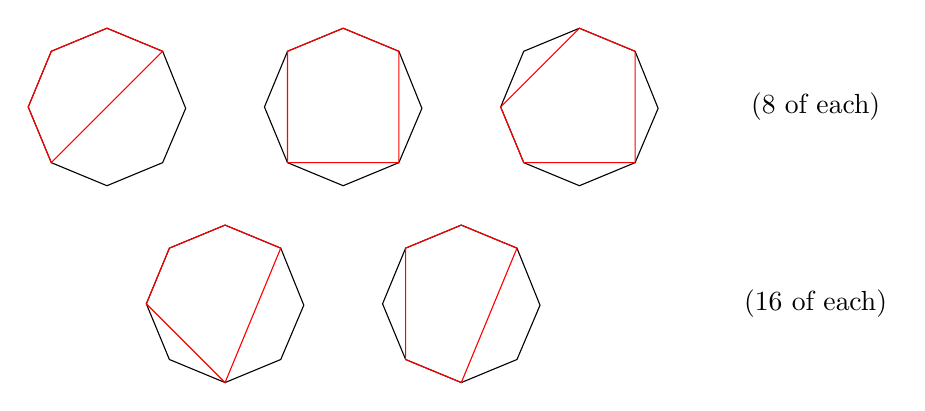
\begin{tikzpicture}
\drawOctagon
\draw[color=red] (P1) -- (P2) -- (P3) -- (P4) -- (P5) -- cycle;
\begin{scope}[xshift=3cm]
\drawOctagon
\draw[color=red] (P1) -- (P2) -- (P3) -- (P5) -- (P7) -- cycle;
\end{scope}
\begin{scope}[xshift=6cm]
\drawOctagon
\draw[color=red] (P1) -- (P2) -- (P4) -- (P5) -- (P7) -- cycle;
\end{scope}
\begin{scope}[yshift=-2.5cm,xshift=1.5cm]
\drawOctagon
\draw[color=red] (P1) -- (P2) -- (P3) -- (P4) -- (P6) -- cycle;
\end{scope}
\begin{scope}[yshift=-2.5cm, xshift=4.5cm]
\drawOctagon
\draw[color=red] (P1) -- (P2) -- (P3) -- (P5) -- (P6) -- cycle;
\end{scope}
\node[] at (9,0) (a) {(8 of each)};
\node[] at (9,-2.5) (a) {(16 of each)};
\end{tikzpicture}
\end{center}

The $A_5$ function is a sum over two of the classes of $A_2$ subalgebras, $x_2\to x_3\left(1+x_4\right)$ and $x_1 \left(1+x_2\right)\to \frac{x_2x_3}{1+x_2}$, appropriately antisymmetrized so that the overall $f_{A_5}$ picks up a minus sign under both $\sigma_{A_5}$ and $\tau_{A_5}$. Explicitly, this is written
\begin{equation}
	f_{A_5} = \sum_{i=0}^7\sum_{j=0}^1(-1)^{i+j}\sigma_{A_5}^i\tau_{A_5}^j\left(\frac12 f_{A_2}\left(x_2\to x_3\left(1+x_4\right)\right) + f_{A_2}\left(x_1 \left(1+x_2\right)\to \frac{x_2x_3}{1+x_2}\right)\right).
\end{equation}
The factor of $\frac12$ in front of $f_{A_2}\left(x_2\to x_3\left(1+x_4\right)\right)$ is simply a symmetry factor, as it lives in an 8-cycle of $\{\sigma_{A_5},\tau_{A_5}\}$.

The two types of $A_2$'s appearing in $f_{A_5}$ are:

\begin{equation}
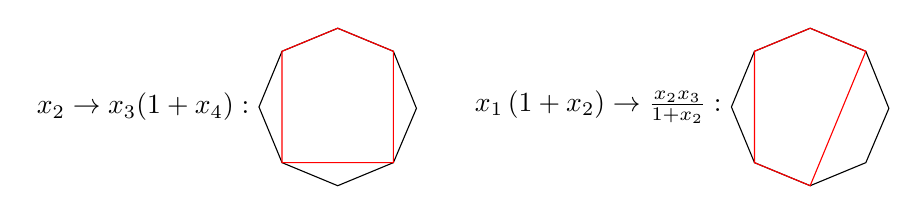
\begin{tikzpicture}
\drawOctagon
\draw[color=red] (P1) -- (P2) -- (P3) -- (P5) -- (P7) -- cycle;
\node[anchor=east] at (-1,0) (a) {$x_2 \to x_3(1+x_4):$};
\begin{scope}[xshift=6cm]
\drawOctagon
\node[anchor=east] at (-1,0) (a) {$x_1 \left(1+x_2\right)\to \frac{x_2x_3}{1+x_2}:$};
\draw[color=red] (P1) -- (P2) -- (P3) -- (P5) -- (P6) -- cycle;
\end{scope}
\end{tikzpicture}
\end{equation}

\section{Conclusion}

\begin{enumerate}
\item since there are so few $D_5$ and $A_5$ subalgebras of Gr(4,7), these decompositions distill more intrinsic (better word?) geometric structure than the $A_3$ function 
\item would be interesting to find the $D_5$ decomposition of higher-point amplitudes, to see if this seter our determined constants
\item not possible to get the full (function-level) amplitude out of a single (function-level) subalgebra function; it merits checking whether a linear combination of different subalgebra functions could be found
\item bring up mutations as active vs passive transformations?
\end{enumerate}

\section*{Acknowledgements}

We thank Jacob Bourjaily, Marcus Spradlin, \dots for illuminating discussions. The authors are grateful to the Kavli Institute for Theoretical Physics (National Science Foundation grant NSF PHY11-25915) for hospitality. 


\appendix

\section{Integrability and Adjacency for \pdfeq{A_2}}  \label{appendix:integrable_A2}

\section{Counting Subalgebras of Finite Cluster Algebras}\label{appendix:subalgebras}
In this appendix we catalog the subalgebra structure for the finite connected cluster algebras \(\subseteq E_6\). These algebras are: \(A_2, A_3, A_4, D_4, A_5, D_5, E_6\).

When counting distinct subalgebras, we lump together all subalgebras which are labeled by the same mutable nodes. However the same subalgebra may appear multiple times but dressed by different frozen nodes -- these appear as distinct subpolytopes in the full associahedra. We have included the counts for both subpolytopes and distinct subalgebras. Also note that in our counting for \xcoords we have included both $x$ and $1/x$.\\ 

{\Large\underline{\(A_2\)}:} \quad clusters: 5 \qquad $a$-coordinates: 5 \qquad $x$-coordinates: 10 \\


{\Large\underline{\(A_3\)}:} \quad clusters: 14 \qquad \(a\)-coordinates: 9 \qquad \(x\)-coordinates: 30 \\

\begin{tabular}{ | l | l | l |}
\multicolumn{1}{c}{Type} &  \multicolumn{1}{c}{Subpolytopes}  &  \multicolumn{1}{c}{Subalgebras} \\
\hline \(A_2\) & 6 & 6 \\ 
\hline \(A_1 \times A_1\) & 3 & 3 \\ 
\hline
\end{tabular} \\ \\


{\Large \underline{\(A_4\)}:} \quad clusters: 42 \qquad \(a\)-coordinates: 14 \qquad \(x\)-coordinates: 70\\ 

\begin{tabular}{ | l | l | l |}
\multicolumn{1}{c}{Type} &  \multicolumn{1}{c}{Subpolytopes}  &  \multicolumn{1}{c}{Subalgebras} \\
\hline \(A_2\) & 28 & 21 \\ 
\hline \(A_1 \times A_1\) & 28 & 28 \\ \hline 
\hline \(A_3\) & 7 & 7 \\ 
\hline \(A_2 \times A_1\) & 7 & 7 \\ 
\hline \(A_1 \times A_1 \times A_1\) & 0 & 0 \\ 
\hline
\end{tabular} \\ \\ 

{\Large\underline{\(D_4\)}:} \quad clusters: 50 \qquad \(a\)-coordinates: 16 \qquad \(x\)-coordinates: 104\\

\begin{tabular}{ | l | l | l |}
\multicolumn{1}{c}{Type} &  \multicolumn{1}{c}{Subpolytopes}  &  \multicolumn{1}{c}{Subalgebras} \\
\hline \(A_2\) & 36 & 36 \\ 
\hline \(A_1 \times A_1\) & 30 & 18 \\ \hline 
\hline \(A_3\) & 12 & 12 \\ 
\hline \(A_2 \times A_1\) & 0 & 0 \\ 
\hline \(A_1 \times A_1 \times A_1\) & 4 & 4 \\ 
\hline
\end{tabular} \\ \\

{\Large\underline{\(A_5\)}:} \quad clusters: 132 \qquad \(a\)-coordinates: 20 \qquad \(x\)-coordinates: 140\\

\begin{tabular}{ | l | l | l |}
\multicolumn{1}{c}{Type} &  \multicolumn{1}{c}{Subpolytopes}  &  \multicolumn{1}{c}{Subalgebras} \\
\hline \(A_2\) & 120 & 56 \\ 
\hline \(A_1 \times A_1\) & 180 & 144 \\ \hline 
\hline \(A_3\) & 36 & 28 \\ 
\hline \(A_2 \times A_1\) & 72 & 72 \\ 
\hline \(A_1 \times A_1 \times A_1\) & 12 & 12 \\ \hline 
\hline \(D_4\) & 0 & 0 \\ 
\hline \(A_4\) & 8 & 8 \\ 
\hline \(A_3 \times A_1\) & 8 & 8 \\ 
\hline \(A_2 \times A_2\) & 4 & 4 \\ 
\hline \(A_2 \times A_1 \times A_1\) & 0 & 0 \\ 
\hline \(A_1 \times A_1 \times A_1 \times A_1\) & 0 & 0 \\ 
\hline
\end{tabular} \\ \\


{\Large\underline{\(D_5\)}:} \quad clusters: 182 \qquad \(a\)-coordinates: 25 \qquad \(x\)-coordinates: 260\\

\begin{tabular}{ | l | l | l |}
\multicolumn{1}{c}{Type} &  \multicolumn{1}{c}{Subpolytopes}  &  \multicolumn{1}{c}{Subalgebras} \\
\hline \(A_2\) & 180 & 125 \\ 
\hline \(A_1 \times A_1\) & 230 & 145 \\ \hline 
\hline \(A_3\) & 70 & 65 \\ 
\hline \(A_2 \times A_1\) & 60 & 50 \\ 
\hline \(A_1 \times A_1 \times A_1\) & 30 & 30 \\ \hline 
\hline \(D_4\) & 5 & 5 \\ 
\hline \(A_4\) & 10 & 10 \\ 
\hline \(A_3 \times A_1\) & 5 & 5 \\ 
\hline \(A_2 \times A_2\) & 0 & 0 \\ 
\hline \(A_2 \times A_1 \times A_1\) & 5 & 5 \\ 
\hline \(A_1 \times A_1 \times A_1 \times A_1\) & 0 & 0 \\ 
\hline
\end{tabular} \\ \\ 

\pagebreak

{\Large\underline{\(E_6\)}:} \quad clusters: 833 \qquad \(a\)-coordinates: 42 \qquad \(x\)-coordinates: 770\\

\begin{tabular}{ | l | l | l |}
\multicolumn{1}{c}{Type} &  \multicolumn{1}{c}{Subpolytopes}  &  \multicolumn{1}{c}{Subalgebras} \\
\hline \(A_2\) & 1071 & 504 \\ 
\hline \(A_1 \times A_1\) & 1785 & 833 \\ \hline 
\hline \(A_3\) & 476 & 364 \\ 
\hline \(A_2 \times A_1\) & 714 & 490 \\ 
\hline \(A_1 \times A_1 \times A_1\) & 357 & 357 \\ \hline 
\hline \(D_4\) & 35 & 35 \\ 
\hline \(A_4\) & 112 & 98 \\ 
\hline \(A_3 \times A_1\) & 112 & 112 \\ 
\hline \(A_2 \times A_2\) & 21 & 14 \\ 
\hline \(A_2 \times A_1 \times A_1\) & 119 & 119 \\ 
\hline \(A_1 \times A_1 \times A_1 \times A_1\) & 0 & 0 \\ \hline 
\hline \(D_5\) & 14 & 14 \\ 
\hline \(A_5\) & 7 & 7 \\ 
\hline \(D_4 \times A_1\) & 0 & 0 \\ 
\hline \(A_4 \times A_1\) & 14 & 14 \\ 
\hline \(A_3 \times A_2\) & 0 & 0 \\ 
\hline \(A_3 \times A_1 \times A_1\) & 0 & 0 \\ 
\hline \(A_2 \times A_2 \times A_1\) & 7 & 7 \\ 
\hline \(A_2 \times A_1 \times A_1 \times A_1\) & 0 & 0 \\ 
\hline \(A_1 \times A_1 \times A_1 \times A_1 \times A_1\) & 0 & 0 \\ 
\hline
\end{tabular}

\section{Cobracket Spaces in Finite Cluster Algebras}\label{appendix:cobrackets}

\bibliographystyle{ieeetr}

\bibliography{subalgebras.bib}

\end{document}
